\documentclass[review]{elsarticle}
% Target journal: Vehicular Communications (Elsevier). Review option = double spaced.
% Compile: pdflatex main.tex
% NUMBER POLICY: every number in this file traces to a results JSON in
%   ../results/ (attack_results_merged.json, train_report.json).
%   Claims not yet backed by a committed artifact are marked [FULL PROTOCOL
%   PENDING] and MUST NOT be unmarked before the run exists. See CLAIMS.md.

\usepackage{amsmath,amssymb}
\usepackage{graphicx}
\usepackage{booktabs}
\usepackage{url}
\usepackage{multirow}
\usepackage{tikz}
\usetikzlibrary{arrows.meta, positioning}

% Marker for claims that await the full-scale protocol runs (3 seeds,
% PGD-50, extended grid, defenses). Greppable: never remove a \FULLP marker
% until the backing result JSON exists in ../results/.
\newcommand{\FULLP}[1]{[\emph{#1 --- full-protocol run pending}]}

\journal{Vehicular Communications}

\begin{document}

\begin{frontmatter}

\title{The Price of Compliance: Emission-Mask-Constrained Adversarial Attacks
on Deep Learning Spectrum Sensing in the 5.9\,GHz ITS Band}

\author[inst1]{Parveen Dhankhar\corref{cor1}}
\ead{parveendhankhar2005@gmail.com}
\author[inst1]{Davesh Vats}
\ead{vatsdavesh@gmail.com}

\cortext[cor1]{Corresponding author.}
\affiliation[inst1]{organization={Department of Computer Science and Engineering,
Vaish College of Engineering},
            city={Rohtak},
            country={India}}

\begin{abstract}
Deep learning (DL) classifiers are increasingly proposed for spectrum sensing
in Vehicle-to-Everything (V2X) networks, and are known to be vulnerable to
adversarial perturbations. Prior wireless adversarial-ML evaluations, however,
either perturb receiver-side features directly---a threat no radio transmitter
can realize---or transmit without regard for spectrum rules. This paper
formalizes and quantifies the attacker that actually exists in the 5.9\,GHz ITS
band: a \emph{compliant attacker} that respects its regulatory allocation and
emission mask while optimizing a waveform-domain perturbation end-to-end
through the attacker-to-receiver channel and the receiver's STFT front-end. We
instantiate the threat model on a post-FCC coexistence sensing task in a
20\,MHz window straddling the 5895\,MHz boundary: C-V2X PC5 and legacy
IEEE~802.11p are co-channel in the ITS band (the transition-period problem),
with U-NII-4 Wi-Fi below the boundary. On TR~37.885-inspired urban, highway,
and rural channels, an unconstrained (``genie'') attacker reaches 20\% conditional attack
success at $-44$\,dB relative received power, while the mask-compliant attacker
needs $-37$ to $-39$\,dB ($-36.7$\,dB under the real ETSI EN 302 571
Table-7 unwanted-emissions template, $-37.4$\,dB when the limits are
enforced in the standard's 1-MHz-RBW mean-power measurement domain, and
in the US 47~CFR~95.3205-shaped limits): an \emph{emission-mask price of
compliance of 5--7\,dB} (6.3--7.5\,dB across all four enforcement
domains; untargeted) and 16--18\,dB for targeted ``cloaking'' of an
active transmitter as noise. The absolute regime is the more alarming finding: an
\emph{undefended} sensing CNN is broken by a rule-abiding transmitter operating
tens of dB below the victim signal level (96.7\% conditional ASR at
$-10$\,dB). We also translate the legacy feature-space threat model into
physical power, showing that receiver-internal $\epsilon$-balls describe a
perturbation that mostly cannot survive its own physical realization, while
a purpose-optimized waveform at the same implied power is far stronger. As the matched defense, mask-matched adversarial training shifts
the compliant-attacker threshold by $+14$\,dB under the evaluation attack
(PGD-10)---but a converged adaptive attack (PGD-50 with random restarts)
recovers most of that margin, leaving $+6.7$\,dB of honestly adaptive
robustness on the canonical defense seed (replicated across three defense
training seeds: $+9.8\pm2.8$\,dB for AT, $+11.5\pm1.8$\,dB for TRADES---the
$3.5$--$5.5$\,dB seed spread is itself a certification finding---and
stable across three attack seeds, $\pm0.1$--$0.7$\,dB; every headline
PoC carries a paired-bootstrap 95\% CI), and the
decomposition attributes the
gap to evaluation step-starvation rather than restart luck. These conclusions are stress-tested beyond the prototype protocol: three
training seeds move the compliant threshold by at most 1.1\,dB;
three-receiver majority fusion buys $+25$\,dB of detection headroom while
leaving the price of compliance unchanged ($6.3$--$7.3$\,dB across $K$);
replacing
the WiFi class with real over-the-air 802.11 captures (recorded at
5.24\,GHz in U-NII-1, the OFDM family adjacent to U-NII-4) replicates the
compliant MEAP within 1.8\,dB while exposing a decision-margin fragility
that synthetic-only evaluation hides entirely; and a second victim
architecture (early-fusion ResNet) shifts the threshold by 11.6--15.1\,dB,
with surrogate-model transfer costing the attacker 11--23\,dB. A
power-amplifier reality check then shows what compliance costs beyond
floating point: the optimized attack waveform has the highest PAPR on the
air (11.1\,dB vs.\ 6.3--9.0\,dB for the classes it impersonates), and a
Rapp-model PA only keeps its post-amplifier spectrum inside a
$-40$\,dBr mask at 13--15\,dB backoff---while the attack itself remains
effective at any backoff, making post-PA regrowth statistics an RF-side
tell against the naive attacker; a PA-aware re-optimization closes even
that tell while gaining 1.2\,dB. The mask idealization itself is then
validated against the real ETSI EN 302 571 Table-7 unwanted-emissions
template: the compliant MEAP moves by only $+0.4$\,dB, so the
price-of-compliance headline is not an artifact of the self-defined mask
shape. Finally, a disclosed-parameter link-budget layer translates the
sensing attack into fleet-scale harm: at the targeted 20\% false-IDLE
operating point a rule-abiding attacker within the 33\,dBm ITS EIRP cap
subtracts 9.4\,pp ($\pm$0.04 over 5 MC seeds) of BSM packet-reception ratio at 100\,m legit-link
distance ($\sim$95 extra lost BSMs per 1000 transmitted). We propose Minimum Effective Attack Power (MEAP) and
Price-of-Compliance (PoC) as physically grounded, transferable security
metrics, and release the complete framework (waveform generators, channels,
attack, defenses, checkpoints, result JSONs with embedded seeds and
configurations) for reproduction.
\end{abstract}

\begin{keyword}
V2X \sep spectrum sensing \sep adversarial machine learning \sep 5.9 GHz
\sep C-V2X \sep IEEE 802.11p \sep emission mask \sep physical-layer security
\end{keyword}

\end{frontmatter}

% ============================================================================
\section{Introduction}
\label{sec:intro}

The 5.9\,GHz ITS band is in the middle of the most consequential spectrum
decision of its history. In FCC~20-164 (2020), the Commission reallocated the
band: the upper 30\,MHz (5895--5925\,MHz) is dedicated to C-V2X, while the
lower 45\,MHz (5850--5895\,MHz) was opened to unlicensed U-NII-4
operation~\cite{fcc2020}; the 2024 Second Report and Order completed the
transition rules and set the DSRC sunset in motion~\cite{fcc2024}. The
transition is no longer prospective: the final rules took effect in
February~2025 with a two-year DSRC sunset, more than fifty waivers already
authorize C-V2X operation in the band~\cite{itsa2024}, and the industry
roadmap projects volume deployment of direct-mode V2X radios in production
vehicles~\cite{5gaa2024}. During and
after this transition, coexistence sensing---determining \emph{which}
technology is transmitting, not merely whether energy is present---becomes a
safety-relevant function: operators of roadside units and vehicles must
distinguish C-V2X
PC5, legacy 802.11p still on the road, and unlicensed Wi-Fi spilling up to the
boundary. Deep learning classifiers are the leading \emph{proposed}
candidate for this
four-way technology recognition---in DAA, coexistence, and O-RAN RIC
designs, though no deployed 2026 radio uses learned sensing
(Section~\ref{sec:standards})---following their success in wireless signal
classification~\cite{o2018,girmay2023}.

The same classifiers, however, inherit the adversarial fragility of deep
networks. A large literature demonstrates that wireless DL classifiers can be
fooled by small, deliberate perturbations~\cite{sadeghi2019,liu2022}. Yet the
threat models in that literature have a physical gap. Feature-space attacks
edit the receiver's input (IQ frames or spectrograms) directly---an adversary
with that access does not need adversarial examples at all. Over-the-air and
channel-aware attacks~\cite{kim2020,sagduyu2021,radioshock2026} closed part of
the gap by transmitting real waveforms through modeled channels, and recent
work has targeted wideband spectrum sensing directly~\cite{zheng2026}. But
none of these asks the question that every real attacker in the 5.9\,GHz band
must answer: \emph{the attacker must obey the very spectrum rules it is
attacking}. A C-V2X device may only transmit in its 10\,MHz ITS allocation
under an emission mask (ETSI EN~302~571~\cite{etsi302571} in Europe; FCC rules
in the US); a U-NII-4 device must stay below 5895\,MHz. An attack that
requires illegal emissions is not an attack on the system---it is a
regulatory violation that conventional spectrum enforcement already handles.

This paper therefore poses and quantifies the \emph{compliant-attacker}
threat model: a spectrum-rule-abiding adversary that transmits only within its
allocation, under an emission mask, with bounded power, while optimizing its
waveform end-to-end through the physical channel and the receiver's
front-end. The question that determines whether mask compliance is itself a
defense is quantitative: \emph{how much attack power does compliance cost?}
We answer it with two new metrics---Minimum Effective Attack Power (MEAP) and
Price of Compliance (PoC)---and with a fully differentiable
waveform$\to$channel$\to$STFT$\to$CNN attack chain whose perturbations are
projected, at every optimization step, onto the physically feasible set.

Our contributions are:
\begin{enumerate}
  \item \textbf{Threat model.} The compliant attacker: an emission-mask and
  allocation constraint on waveform-domain adversarial perturbations, to our
  knowledge the first such constraint in the wireless adversarial-ML
  literature (Table~\ref{tab:threat}).
  \item \textbf{Task.} A post-FCC coexistence sensing benchmark in a
  20\,MHz window straddling the 5895\,MHz boundary: block-exact 802.11p and
  U-NII-4 generators and a rate-matched C-V2X PC5 generator, co-channel
  802.11p/PC5 in the ITS allocation (the transition problem), with an
  honest energy-feature baseline showing where deep learning is and is not
  needed.
  \item \textbf{Attack.} A differentiable projected-gradient attack over the
  waveform, with out-of-band nulling, an in-band PSD cap, and an explicit
  power budget defined as the physical attack-to-signal power ratio (PSR).
  \item \textbf{Metrics.} MEAP and PoC: power-domain, attacker-agnostic
  robustness measures suitable for certification-style reporting.
  \item \textbf{Findings.} On TR~37.885-inspired channels: compliance costs
  the attacker ${\sim}5$--7\,dB (untargeted) and 16--18\,dB (targeted
  cloaking); an undefended CNN is nevertheless broken by a compliant attacker
  at deeply negative PSR; the legacy feature-space $\epsilon$-ball assumes a
  hidden power budget we make measurable; and mask-matched adversarial
  training shifts the compliant-attacker threshold by $+14$\,dB under the
  evaluation attack ($+6.7$\,dB against the converged adaptive attack on the
  canonical defense seed; $+9.8\pm2.8$\,dB across three defense seeds;
  Section~\ref{sec:adaptive}) at no
  clean-accuracy cost. Compliance \emph{delays} the attack; so does the
  defense; neither prevents it.
\end{enumerate}

\paragraph{Scope and honesty} All attack numbers in this paper are
prototype-scale (three training seeds for the undefended headline, two
attack seeds, 300 evaluation windows, PGD-10) and are labeled as such; the
full protocol (PGD-50, extended grid) is specified in the released
repository; rural, PGD-50, a second attack seed, the mask-cap sensitivity,
the defense study, the feature-space comparison, real over-the-air
captures, a second victim architecture, and surrogate-model transfer are
included here. Every number traces to a result JSON with embedded
configuration. The undefended model is
the subject of Sections~\ref{sec:poc}--\ref{sec:featurespace}; the defense
study (Section~\ref{sec:defenses}) quantifies how much of the threat
adversarial training removes.

\section{Related Work and Threat-Model Positioning}
\label{sec:related}

\paragraph{DL spectrum sensing and ITS-band recognition} Deep learning radio
signal classification was established at scale by O'Shea et
al.~\cite{o2018}. For the ITS band specifically, Girmay et
al.~\cite{girmay2023} built CNN-based technology recognition and traffic
characterization for coexisting wireless technologies---the coexistence
problem our task generator mirrors. These works establish capability, not
robustness.

\paragraph{Adversarial attacks on wireless DL} Sadeghi and
Larsson~\cite{sadeghi2019} demonstrated white-box attacks on modulation
classifiers in feature space. Liu et al.~\cite{liu2022} attacked
spectrum sensing in cognitive-radio IoT, again at the feature level.
Over-the-air reality was first confronted by Kim et al.~\cite{kim2020} and
matured into channel-aware attacks~\cite{sagduyu2021}, which optimize the
transmit waveform through a modeled channel; RadioShock~\cite{radioshock2026}
demonstrated OTA attacks with channel-state estimation, and Zheng et
al.~\cite{zheng2026} brought targeted attacks to wideband spectrum sensing.
Defense-side, Zhao et al.~\cite{zhao2024} proposed statistical detection of
adversarial spectrum attacks, and Croce and Hein~\cite{croce2020} established
reliable attack ensembles for robustness evaluation. In the standards world,
Habler et al.~\cite{habler2025} mapped adversarial-ML threats onto O-RAN
architectures---the deployment context our metrics target.

\paragraph{Primary-user emulation: the pre-DL ancestor} Constraining the
\emph{attacker} rather than its perturbation has a long history in a
neighboring community. Primary-user-emulation attacks (PUEA)---a malicious
node transmitting so that energy-detection sensors believe the primary user
is present (denial of service) or absent (spectrum theft)---were formalized
by Anand et al.~\cite{anand2008} and remain an active detection
literature~\cite{ambhika2024}. PUEA and the compliant attacker share one
premise---the adversary transmits a real waveform---but differ in everything
downstream: the victim (an occupancy threshold vs.\ a deep classifier), the
mechanism (statistical mimicry of the primary's signal and power geometry
vs.\ a gradient-optimized perturbation through the receiver's
front-end), the constraint set (attacker power and distance, but no
allocation or emission-mask constraint, vs.\ the regulatory feasible set
here), and the reported quantities (occupancy error rates vs.\ power-domain
robustness metrics). The compliant-attacker threat model is not a
rediscovery of PUEA; it is its adversarial-ML descendant, inheriting the
``real waveform, real power budget'' premise while replacing the victim,
the optimization, and the measurement.

\paragraph{Positioning} Table~\ref{tab:threat} positions the compliant
attacker. The differentiator is not ``channel awareness'' (present
in~\cite{sagduyu2021,radioshock2026}) nor the sensing task
(present in~\cite{liu2022,zheng2026}); it is the \emph{regulatory constraint
set}: allocation, emission mask, and an explicit power budget swept as the
independent variable. To our knowledge no prior work constrains a wireless
adversary to its spectrum rules, and none reports a power-domain
price-of-compliance analysis. This matters because compliance is the one
attacker property that is \emph{verifiable by regulators}: an attacker that
must obey the mask is within the reach of conformance testing, which makes
the resulting robustness metrics deployable (Section~\ref{sec:standards}).

\begin{table}[t]
\centering
\caption{Threat-model comparison. ``Mask'' = regulatory allocation +
emission-mask constraint on the transmitted adversarial perturbation.
PUEA = primary-user emulation, the pre-DL ancestor (Section~\ref{sec:related}).
``Power sweep'': \emph{fixed} = single power level; \emph{PNR} = accuracy-vs-PNR
sweeps with no threshold-in-power metric; \emph{MEAP} = threshold-in-power
robustness metric (this work).}
\label{tab:threat}
\small
\begin{tabular}{lccccc}
\toprule
Work & Waveform & Channel & Mask & Power sweep & Task \\
\midrule
Sadeghi \& Larsson~\cite{sadeghi2019} & -- & -- & -- & -- & modulation \\
Liu et al.~\cite{liu2022} & -- & -- & -- & -- & spectrum sensing \\
Anand et al.~\cite{anand2008} (PUEA) & \checkmark & -- & -- & fixed & occupancy \\
Kim et al.~\cite{kim2020} & \checkmark & \checkmark & -- & fixed & modulation \\
Kim et al.~\cite{sagduyu2021} & \checkmark & \checkmark & -- & PNR & modulation \\
Zheng et al.~\cite{zheng2026} & \checkmark & \checkmark & -- & fixed & wideband sensing \\
RadioShock~\cite{radioshock2026} & \checkmark & \checkmark & -- & fixed & communication \\
\textbf{This work} & \checkmark & \checkmark & \textbf{\checkmark} & \textbf{MEAP} & \textbf{ITS coexistence} \\
\bottomrule
\end{tabular}
\end{table}

\section{System Model}
\label{sec:system}

\subsection{Post-FCC coexistence sensing task}
\label{sec:task}

The sensing receiver observes a 20\,MHz complex-baseband window
(2048 samples at $F_S = 20$\,MHz, i.e., 102.4\,\textmu s) centered on the
5895\,MHz boundary, covering 5885--5905\,MHz (Fig.~\ref{fig:bandplan}). This
boundary-straddling placement is the physically interesting vantage point:
the upper half contains the ITS allocation (5895--5905\,MHz is the lowest
C-V2X channel), the lower half the upper edge of U-NII-4 unlicensed
operation. The classification task is four-way (Table~\ref{tab:bandplan}):

\begin{figure}[t]
\centering
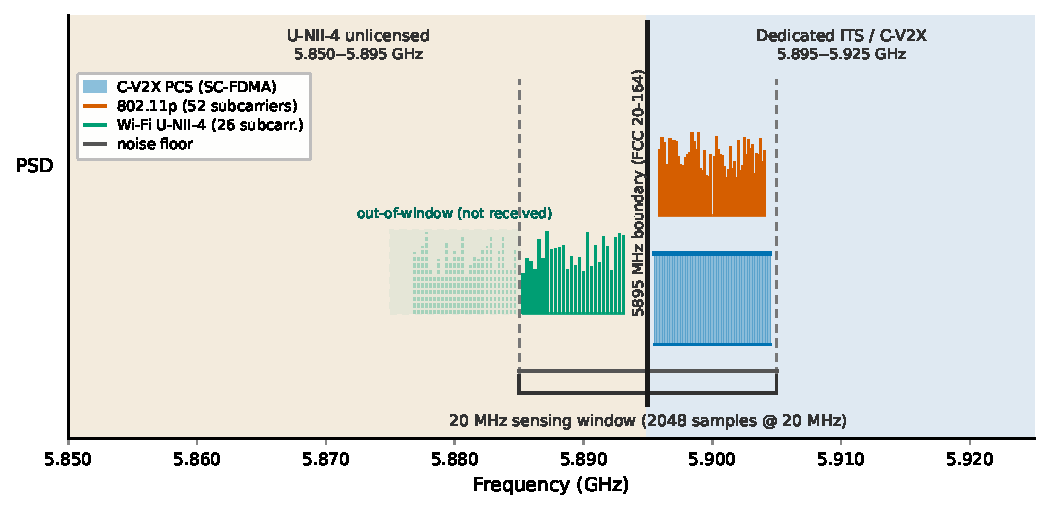
\includegraphics[width=0.98\linewidth]{figs/band_plan.pdf}
\caption{Post-FCC 5.9\,GHz band plan as seen by the boundary-straddling
sensing window (stylized PSD, not to scale). Shading marks the two
regulatory blocks created by FCC~20-164: unlicensed U-NII-4 below the
5895\,MHz boundary and the dedicated ITS/C-V2X allocation above it. C-V2X
PC5 (flat-topped SC-FDMA block) and IEEE~802.11p (52 raised subcarrier
stems) are deliberately co-channel in the lowest 10\,MHz ITS channel; the
Wi-Fi class is the partial 26-subcarrier view of a U-NII-4 channel centered
10\,MHz below the window, whose out-of-window half (dashed ghost) is removed
by the receiver's anti-alias filter.}
\label{fig:bandplan}
\end{figure}

\begin{table}[h]
\centering
\caption{Post-FCC band plan as seen by the sensing window (frequencies
relative to the 5895\,MHz boundary). PC5 and 802.11p are deliberately
co-channel: the transition-period coexistence problem.}
\label{tab:bandplan}
\small
\begin{tabular}{llll}
\toprule
Class & Standard basis & Occupied (MHz) & Generation \\
\midrule
C-V2X PC5 & Rel-14 SC-FDMA$^{\dagger}$ & $[+0.5, +9.5]$ & contiguous DFT-s-OFDM \\
802.11p & 802.11-2012 OFDM & $[+0.94, +9.06]$ & 52-sub IFFT+CP, DC nulled \\
Wi-Fi U-NII-4 & 802.11 20\,MHz OFDM & $[-9.69, -1.88]$ & 26 in-window subcarr. \\
Noise & -- & full band & complex AWGN \\
\bottomrule
\multicolumn{4}{l}{\footnotesize $^{\dagger}$rate-matched stylization: 450$\times$20\,kHz
(9\,MHz = Rel-14 occupied BW); SCS/DMRS not modeled (Sec.~\ref{sec:limitations}).}
\end{tabular}
\end{table}

Two design decisions deserve justification. First, \emph{802.11p and PC5 are
co-channel} in the ITS allocation: during the multi-year DSRC sunset,
roadside infrastructure must classify both technologies sharing the same
spectrum, and region-energy features reliably cannot separate them---our
logistic-regression baseline on region-energy and envelope features reaches
only 77.75\% on this pair, while the CNN reaches 100\% (four-class baseline:
88.62\% vs 100\%). The DL-necessity claim is thus confined to what physics
cannot do, unlike prior work where classes are region-separable and
``deep learning needed'' claims do not survive an energy baseline. Second,
\emph{Wi-Fi is region-separable from the ITS pair} (it lives below the
boundary); this is correct post-FCC physics, and we state it rather than
engineer it away.

The waveform generators are block-exact where the standards allow it at
$F_S=20$\,MHz: 802.11p~\cite{ieee80211} uses 52 subcarriers at 156.25\,kHz spacing with a
1.6\,\textmu s cyclic prefix and a nulled DC subcarrier; the U-NII-4 class is
the physically correct partial view of a 20\,MHz 802.11 channel (312.5\,kHz
spacing, 0.8\,\textmu s guard interval) whose center lies 10\,MHz below the
window---only the 26 in-window subcarriers are generated, as the receiver's
anti-alias filter removes the rest. PC5 is a rate-matched stylization of
Rel-14~\cite{ts36211}: 450 subcarriers at 20\,kHz (the same 9\,MHz occupied
bandwidth as 50 PRBs at 15\,kHz), chosen so the block is an exact integer at
$F_S=20$\,MHz; single-carrier structure and PAPR are preserved (measured:
6.26\,dB PC5 vs 8.77/8.69\,dB for the OFDM classes, matching the committed
benign-PAPR statistics in our PA reality-check data). All data symbols are
QPSK; pilots and preambles are not modeled.

\subsection{Channel model}
\label{sec:channels}

Channels are simplified, TR~37.885-inspired~\cite{tr37885} block-fading
tapped-delay models: highway (120\,km/h, Rician $K=10$\,dB first tap, 5
taps, ${\sim}$0.4\,\textmu s spread), urban (50\,km/h, Rayleigh, 6 taps,
${\sim}$1.3\,\textmu s spread, UMa-flavored), and rural (30\,km/h, $K=5$\,dB,
3 taps). Block fading is justified even at highway speed: the maximum Doppler
(${\sim}$656\,Hz at 5.9\,GHz) gives a decorrelation time of
${\sim}$0.55--0.76\,ms, far exceeding the 102.4\,\textmu s window. The
victim link and the attacker-to-receiver link draw independent channel
realizations. Deviations from the spec's CDL profiles (first-tap-only
Rician, UMa-flavored urban spread) are disclosed in
Section~\ref{sec:limitations}.

\subsection{Receiver front-end and classifier}
\label{sec:frontend}

The receiver computes a complex STFT (256-point, 128 hop, Hann window,
two-sided and frequency-shifted) yielding $256\times15$ frames, from which
two streams are derived: log-magnitude (z-scored, clamped) and the per-bin
temporal phase difference (a phase-vocoder-style frequency-offset estimate).
Both streams feed a dual-stream Inception-Time CNN (86,052 parameters),
carried over from our prior work~\cite{dhankhar2026} for architectural
comparability; a magnitude-only variant (40,980 parameters) serves as the
pre-registered stream ablation. The entire chain is implemented in PyTorch
and is differentiable end-to-end from time-domain waveform to logits---the
enabler of the waveform-domain attack. Training uses the prior work's recipe
(label smoothing 0.1, TF-CutMix, Gaussian augmentation, Adam 5e-4, cosine
schedule) on 3,200 training windows (800 held-out validation windows) with
mixed scenarios and SNR drawn uniformly from [5,~25]\,dB.

\section{The Compliant Attacker}
\label{sec:attack}

\begin{figure}[t]
\centering
\resizebox{\textwidth}{!}{%
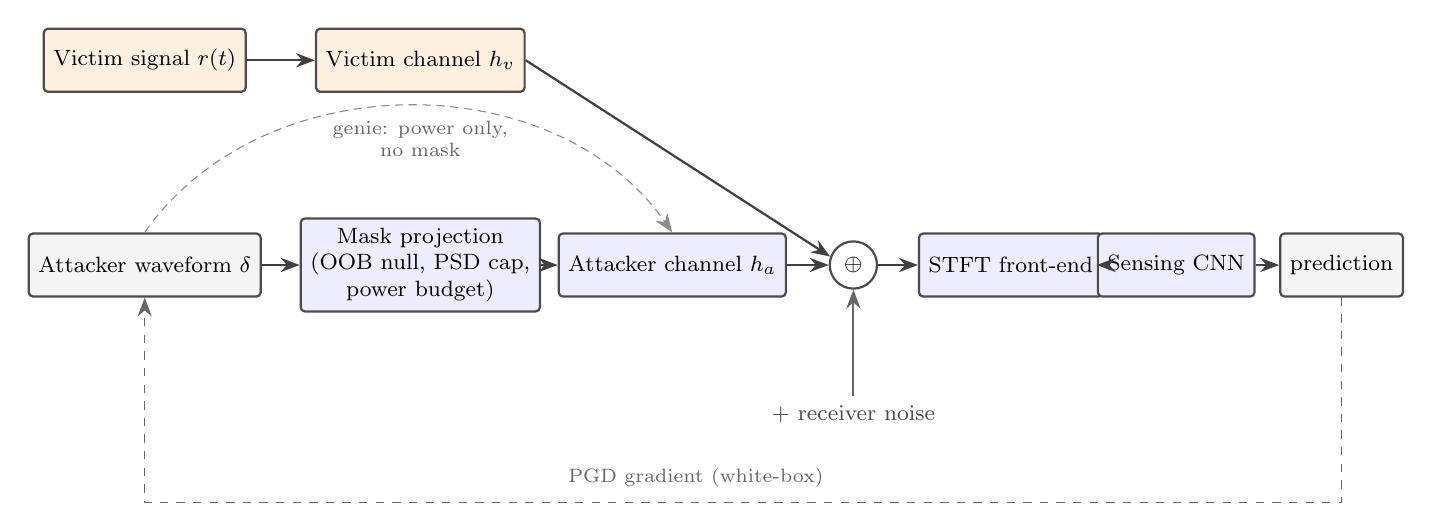
\begin{tikzpicture}[
  font=\footnotesize,
  box/.style={draw=black!70, thick, rounded corners=1.5pt, align=center,
              inner sep=3.5pt, minimum height=8mm},
  io/.style={box, fill=black!4},
  atk/.style={box, fill=blue!7},
  vic/.style={box, fill=orange!12},
  arr/.style={-{Stealth[length=2.4mm]}, thick, black!75},
  fb/.style={-{Stealth[length=2.4mm]}, dashed, black!60},
  gen/.style={-{Stealth[length=2.4mm]}, densely dashed, black!45},
]
% attacker chain (middle row)
\node[io] (delta) at (0,0) {Attacker waveform $\delta$};
\node[atk] (mask) at (3.5,0) {Mask projection\\(OOB null, PSD cap,\\power budget)};
\node[atk] (ha) at (6.7,0) {Attacker channel $h_a$};
\node[circle, draw=black!70, thick, minimum size=6mm, inner sep=0pt]
  (sum) at (9.0,0) {$\oplus$};
\node[atk] (stft) at (11.0,0) {STFT front-end};
\node[atk] (cnn) at (13.1,0) {Sensing CNN};
\node[io] (pred) at (15.2,0) {prediction};
% victim path (top row) joins the same junction
\node[vic] (victim) at (0,2.6) {Victim signal $r(t)$};
\node[vic] (hv) at (3.5,2.6) {Victim channel $h_v$};
% receiver noise into the junction
\node[black!70] (noise) at (9.0,-1.9) {$+$ receiver noise};
% arrows: attacker chain
\draw[arr] (delta) -- (mask);
\draw[arr] (mask) -- (ha);
\draw[arr] (ha) -- (sum);
\draw[arr] (sum) -- (stft);
\draw[arr] (stft) -- (cnn);
\draw[arr] (cnn) -- (pred);
\draw[arr] (victim) -- (hv);
\draw[arr] (hv.east) -- (sum.160);
\draw[arr, black!60] (noise) -- (sum.270);
% genie bypass: power only, no mask
\draw[gen] (delta.north) to[out=55,in=125] (ha.north);
\node[black!60, align=center, font=\scriptsize] at (3.5,1.6)
  {genie: power only,\\no mask};
% PGD feedback (white-box)
\draw[fb] (pred.south) -- ++(0,-2.6) -| (delta.south);
\node[black!60, anchor=south, font=\scriptsize] at (7.0,-2.95)
  {PGD gradient (white-box)};
\end{tikzpicture}%
}
\caption{Threat model of the compliant attacker. The attacker optimizes a
waveform-domain perturbation $\delta$ end-to-end through its own channel
$h_a$, the receiver's STFT front-end, and the sensing CNN; the dashed
return path carries the white-box PGD gradient. The \emph{compliant}
variant projects $\delta$ onto the feasible set (out-of-band null, in-band
PSD cap, transmit-power budget) at every optimization step, while the
\emph{genie} variant bypasses the mask projection and obeys only the power
budget. The victim signal $r(t)$ arrives through an independent channel
$h_v$; the junction also adds receiver noise.}
\label{fig:threat}
\end{figure}

\subsection{Threat model}
\label{sec:threatmodel}

The adversary is a C-V2X device transmitting in its own ITS allocation
$[0,+10]$\,MHz relative to the boundary. Its perturbation $\delta \in
\mathbb{C}^{N}$ must satisfy, \emph{at its transmit port}:
(i) \emph{allocation}: $\mathrm{supp}(\hat{\delta}) \subseteq
\mathcal{B}_a$ (out-of-band FFT bins nulled);
(ii) \emph{emission mask}: $|\hat{\delta}_k|^2 \le M_k$ in-band (a flat PSD
cap at $2\times$ uniform budget sharing---an idealization stricter than real
in-band regulations, whose sensitivity we report); and
(iii) \emph{power}: $\|\delta\|_2^2 \le P_a$, with the physical budget
expressed as PSR~(dB) $= 10\log_{10}(E_{\mathrm{attack}} /
E_{\mathrm{clean\,rx}})$ over equal-length windows---the ratio of adversarial
transmit power to received victim-signal power. A \emph{genie} baseline
obeys only (iii): the classical unrestricted upper bound. The attacker knows
the victim model and its own attacker-to-receiver channel (white-box with
CSI); \emph{worst-case disclosure}: the optimization also uses the exact
received realization (signal + noise), so all reported ASRs are upper
bounds---the direction favorable to the attack. Section~\ref{sec:poc}
quantifies how this degrades under CSI error and with no CSI at all.
Figure~\ref{fig:threat} summarizes
the attack chain and the two attacker variants.

\subsection{Feasible set and projected-gradient attack}
\label{sec:pgd}

\begin{equation}
\mathcal{F} = \{\delta \in \mathbb{C}^{N} :
\mathrm{supp}(\hat{\delta}) \subseteq \mathcal{B}_a,\;
|\hat{\delta}_k|^2 \le M_k,\;
\|\delta\|_2^2 \le P_a \}
\label{eq:feasible}
\end{equation}

The attack optimizes $\delta$ by PGD through the differentiable chain
$\delta \rightarrow h_a \ast \delta \rightarrow + r(t) \rightarrow
\mathrm{STFT} \rightarrow \mathrm{CNN} \rightarrow \mathcal{L}$, with
loss $\mathcal{L} = -\mathrm{CE}$ (untargeted) or $\mathrm{CE}(\cdot,
y_{\mathrm{target}}=\mathrm{Noise})$ (targeted ``cloaking'': make an active
transmitter look like an idle band). After each step, $\delta$ is projected
onto $\mathcal{F}$: FFT-domain out-of-band nulling, per-bin PSD capping
(Parseval-corrected: $\sum_k |\hat{\delta}_k|^2 = N \|\delta\|_2^2$), and
total-power rescaling. The projection is exactly idempotent and enforces the
budget to machine precision (verified: post-projection power ratio
$1.000000$, out-of-band fraction $10^{-14}$). Compliance is defined at the
transmit port; the finite sensing window spreads the \emph{received}
adversarial component to ${\sim}-33.5$\,dB out-of-band fraction---a receiver
artifact, not a transmit violation.

\subsection{Physical security metrics}
\label{sec:metrics}

Raw ASR conflates attack success with the classifier's base error; we
report \emph{conditional ASR} over clean-correctly-classified windows, and
\emph{robust accuracy} over all windows. Two power-domain metrics summarize
the threat: \emph{MEAP} (Minimum Effective Attack Power) is the PSR at which
conditional ASR crosses 20\% (linear interpolation, with explicit censoring
flags when the grid does not resolve the crossing); \emph{Price of
Compliance} is $\mathrm{PoC} = \mathrm{MEAP}_{\mathrm{compliant}} -
\mathrm{MEAP}_{\mathrm{genie}}$: the power a rule-abiding attacker must
additionally spend to achieve the same attack success. PoC is
budget-matched, attacker-agnostic, and---unlike ASR at a fixed
$\epsilon$---directly interpretable in link-budget terms.

\section{Experimental Evaluation}
\label{sec:experiments}

\subsection{Protocol and scale}
\label{sec:protocol}

Unless stated otherwise, every experiment below uses the same evaluation
contract: a frozen victim model, a fixed set of active-transmission windows
(PC5, 802.11p, WiFi), per-sample attacker channels drawn from the scenario
model, and the PSR grid of Table~\ref{tab:protocol}; conditional ASR is
measured only over windows the victim classified correctly before the
attack, and every MEAP carries an explicit censoring flag when the grid
does not resolve it. Every conditional-ASR cell is stored with its
success count and eligibility, and headline MEAP/PoC numbers carry
Wilson binomial 95\% confidence intervals (sampling noise at fixed
model/protocol; model-seed spread is reported separately); because the
genie and mask arms attack the \emph{same} windows, headline PoCs
additionally carry paired-bootstrap 95\% CIs
(Section~\ref{sec:adaptive}) that propagate the shared sampling noise
instead of worst-casing each arm separately. The honesty box records the prototype scale; the
three-seed statistics, PGD-50 convergence, adaptive (multi-restart)
evaluation of the defenses, and sensitivity checks in
Section~\ref{sec:poc} quantify how far the prototype numbers generalize.

\begin{table}[h]
\centering
\caption{Protocol honesty box. Prototype-scale numbers in this paper use the
first row; the full protocol is released with the repository.}
\label{tab:protocol}
\small
\begin{tabular}{ll}
\toprule
Setting & Value (prototype) \\
\midrule
Training & seeds 42/123/456 (undefended headline), 3{,}200 train / 800 val windows, SNR [5,25]\,dB; defenses seed 42 + replication seeds 43/53 (adaptive margins, 3-seed) \\
Attack & seed 7, 300 active-tx windows, PGD-10, $\alpha=0.25$ \\
Adaptive attack & PGD-50, 5 restarts (zero-init + 4 random), best-of-R per sample; 3 defense seeds \\
PSD cap margin & 2.0 (flat-cap idealization; relaxing to 10 moves PoC by $-0.9$\,dB) \\
PSR grid & $-45$ to $+10$\,dB, 12 points \\
MEAP threshold & 20\% conditional ASR \\
Confidence & Wilson 95\% binomial CIs on every ASR cell; paired-bootstrap MEAP/PoC CIs (results/w12\_confidence\_intervals.json, results/w14b\_bootstrap\_cis.json) \\
\bottomrule
\end{tabular}
\end{table}

\subsection{Clean sensing performance}
\label{sec:clean}

The dual-stream CNN and the magnitude-only ablation both reach 100\%
validation accuracy (800 held-out windows); the energy-feature logistic
regression baseline reaches 88.62\% (four-class) and 77.75\% on the
co-channel PC5-vs-802.11p pair, where the CNN is error-free. Across the
three training seeds (42/123/456) the picture is stable: clean accuracy is
100\% for all seeds, the LR baseline moves within one point
(88.6/88.1/87.8\%), and the LR pair accuracy spreads 74.0--77.8\%
(mean 76.3\%) while the CNN pair stays error-free throughout. The phase
difference stream contributes nothing (dual = mag-only), retiring the
``phase-aware'' framing of our prior work~\cite{dhankhar2026}---an honest
negative result, pre-registered as an ablation. An SNR sweep below the training
range bounds the noise-floor regime honestly: the CNN's advantage over the
energy baseline persists down to 0\,dB SNR (71.8\% vs 61.3\% at
$[0,10]$\,dB, 63.2\% on the hard pair) and vanishes at negative SNR
(24.3\% vs 25.0\% at $[-10,0]$\,dB)---both models starve; deep learning
does not rescue a task with no signal. (The first version of this sweep
drew its evaluation baseband from the training seed's RNG stream; a
hash-level audit found $2/1000$ realized waveforms bit-identical to
training-corpus members. The numbers above use a fresh evaluation seed
verified at $0/1000$ overlap; every accuracy moved by at most
$1.3$\,pp, within sampling noise at $n{=}1000$---the leak was real but
immaterial, and both the audit and the clean re-run are released.)

\subsection{The price of compliance}
\label{sec:poc}

\begin{figure}[t]
\centering
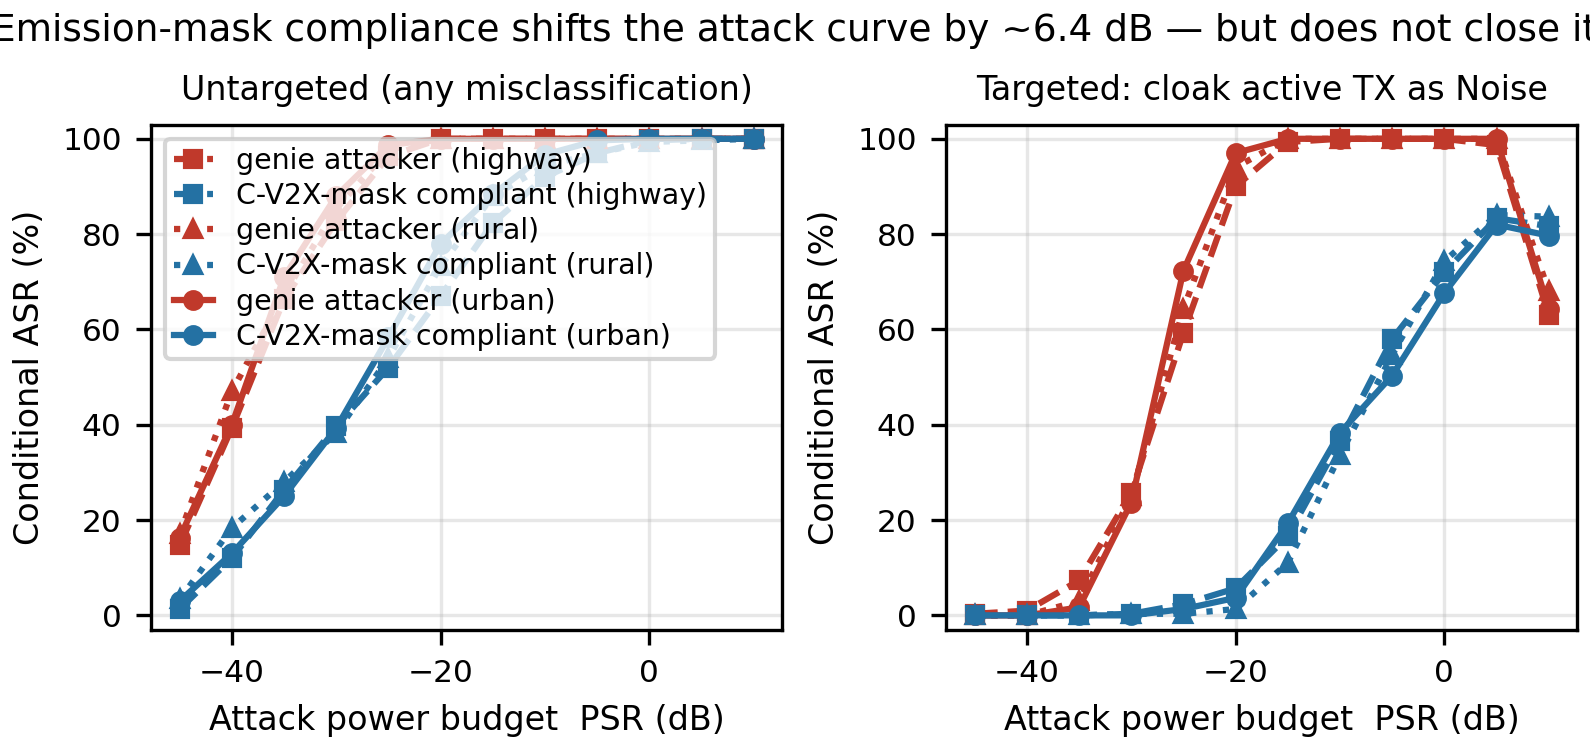
\includegraphics[width=0.95\linewidth]{figs/price_of_compliance.png}
\caption{Conditional ASR versus attack power budget (PSR, dB) for genie vs
emission-mask-compliant attackers, untargeted and targeted-to-Noise modes,
urban, highway, and rural channels (prototype protocol of
Table~\ref{tab:protocol}). Compliance shifts the attack curve right by
${\sim}$5--7\,dB (untargeted) but does not close it; both attackers break the
undefended CNN at deeply negative PSR.}
\label{fig:poc}
\end{figure}

\begin{table}[t]
\centering
\caption{Physical summary metrics (conditional-ASR threshold 20\%;
prototype protocol of Table~\ref{tab:protocol}; all MEAPs resolved within
the grid, no censoring). Training-seed stability (seeds 42/123/456, urban
untargeted): compliant MEAP $-37.1/-38.1/-37.9$\,dB (mean $-37.7$, spread
1.1\,dB); genie MEAP at or below the grid floor for 2 of 3 seeds, so the
per-seed PoC (7.1/6.9/7.1\,dB) is a lower bound for those seeds. The
compliant column uses the idealized flat-cap mask; under the real ETSI
EN 302 571 Table-7 template the urban untargeted row becomes $-36.7$\,dB
MEAP, PoC $7.5$\,dB, and $-37.4$\,dB / PoC $6.9$\,dB when the limits are
enforced in the clause-6.4.2-style 1-MHz-RBW mean-power measurement domain
(Sections~\ref{sec:etsimask}--\ref{sec:conformance}).}
\label{tab:metrics}
\begin{tabular}{llrrr}
\toprule
Scenario & Mode & MEAP genie & MEAP compliant & Price of Compliance \\
\midrule
urban & untargeted & $-44.2$ dB & $-37.1$ dB & $7.1$ dB \\
highway & untargeted & $-43.9$ dB & $-37.2$ dB & $6.7$ dB \\
rural & untargeted & $-44.5$ dB & $-39.1$ dB & $5.4$ dB \\
urban & targeted-noise & $-30.8$ dB & $-14.8$ dB & $16.0$ dB \\
highway & targeted-noise & $-31.5$ dB & $-14.2$ dB & $17.4$ dB \\
rural & targeted-noise & $-31.1$ dB & $-13.0$ dB & $18.1$ dB \\
\bottomrule
\end{tabular}
\end{table}

Four findings emerge (Fig.~\ref{fig:poc}, Table~\ref{tab:metrics}).
\textbf{(F1) Undefended CNNs are catastrophically
brittle in absolute terms.} The genie attacker reaches 20\% conditional ASR
at $-44$\,dB---four orders of magnitude below the received signal---and the
\emph{compliant} attacker at $-37$\,dB. At $-10$\,dB (an attacker ten times
weaker than the victim signal), the compliant attacker achieves 96.7\%
(urban) / 92.0\% (highway) conditional ASR, and 39.3\% (urban) /
39.7\% (highway) even at $-30$\,dB. \textbf{(F2) Compliance costs
${\sim}$5--7\,dB} for generic misclassification, consistently across urban,
highway, and rural channels---the price is a property of the mask, not the
channel. \textbf{(F3) Cloaking is the costlier attack:} forcing the specific
``Noise'' label costs the compliant attacker 16--18\,dB more than the genie
(0.4\% or less conditional ASR below $-25$\,dB; 38.3\%/36.7\% at
$-10$\,dB; 68\%/72\% at parity).
Target specificity, not generic misclassification, is where the mask bites.
\textbf{(F4) Overshoot at high power:} at $+10$\,dB the targeted attack's
Noise-specific success \emph{decreases} (genie 63--68\%, compliant
80--84\%) while untargeted damage saturates---the perturbation overshoots
into other wrong classes (robust accuracy is 8--14\%), a real phenomenon for certified-decision pipelines
that key on specific labels.

\paragraph{Robustness of the metrics} Three checks bound the main threats to
validity of Table~\ref{tab:metrics}. \emph{Attack-strength convergence:}
PGD-50 (versus PGD-10) shifts the compliant MEAP by only $-1.7$\,dB (to
$-38.8$\,dB; its genie MEAP is censored at that grid's floor) and raises
mid-grid conditional ASR substantially (up to $+37$\,pp at $-25$\,dB)---the
zero-initialized, restart-free PGD-10 protocol therefore reports materially
\emph{conservative} attack numbers, and the PGD-10 MEAPs are lower bounds.
\emph{Seed stability:} a second attack
seed (11) reproduces the urban untargeted PoC at 6.9\,dB versus 7.1\,dB
(0.3\,dB spread; MEAPs move by $\le$1\,dB). \emph{Mask-cap idealization:}
relaxing the flat in-band cap from $2\times$ to $10\times$ uniform sharing
moves the compliant MEAP by only $-0.9$\,dB and the PoC from 7.1 to
6.2\,dB---the Price of Compliance is driven by the \emph{allocation}
constraint (the out-of-band null), not by how strictly in-band flatness is
enforced. \emph{Attacker knowledge:} re-running the compliant attack with
imperfect CSI (additive error of 0.3 relative magnitude) costs at most
2.7\,pp of conditional ASR across the measured grid---the attack is robust
to CSI error; but with \emph{no} CSI (optimizing against
an independent draw from the same scenario, evaluated on the true channel)
the compliant attack's 20\%\,ASR threshold moves from $-37$\,dB to
$\approx\!-16$\,dB, a $\sim$21\,dB penalty: channel-realization
knowledge, not channel statistics, is what makes the white-box threat
catastrophic. \emph{Training-seed statistics:} retraining the victim from
scratch on seeds 123 and 456 (identical recipe) and re-running the full
urban untargeted grid gives compliant MEAPs of $-38.1$ and $-37.9$\,dB
against seed~42's $-37.1$\,dB---a 1.1\,dB total spread, with clean
accuracy 100\% and the CNN pair error-free on every seed. The genie MEAP
falls at or below the $-45$\,dB grid floor for the two new seeds, making
their PoCs lower bounds (6.9 and 7.1\,dB); the ordering genie~$<$~compliant
threshold, and the ${\sim}$7\,dB price of compliance, are invariant to
the training seed.

\subsection{What the legacy feature-space threat model silently assumes}
\label{sec:featurespace}

A log-magnitude perturbation of $\pm\epsilon$ (in z-scored units) in the
receiver's spectrogram has no direct physical meaning. It can be given one:
a log-magnitude change $d$ on bin $k$ corresponds to the complex STFT-domain
addition $\hat{\Delta}_k = \hat{Z}_k (10^{d} - 1)$ (magnitude scaling, phase
preserved), and the hann/50\%-overlap STFT is invertible (interior
reconstruction error $8.4\times10^{-7}$), so the same edit implies a
\emph{received} waveform perturbation whose power we can measure
(PSR$_{\mathrm{eq}}$). We attack the magnitude input with an
$\ell_\infty$ PGD ($\epsilon \in \{0.1, 0.3, 1.0\}$) and translate the
perturbation to the waveform domain. At $\epsilon = 1.0$ (one standard
deviation of the log-magnitude distribution) the feature-space attack
achieves 71.3\% conditional ASR \emph{as evaluated in the legacy setting}
(the perturbed spectrogram is fed directly to the CNN), while its implied
received power is $-24$\,dB (median). Feeding the actual waveform
$x + \delta_{\mathrm{rx}}$ through the receiver's true front-end realizes
only 14.0\%: the hann-window round trip realizes roughly half of the
intended per-bin log-change, and the receiver noise absorbs the rest. By
contrast, \emph{transmitted} attacks optimized for that same power
($-24$\,dB) achieve 99.3\% (genie) and 62.3\% (compliant). At
$\epsilon = 0.3$ the legacy attack achieves 1.7\% intended (0\%
realized) at an implied $-34.4$\,dB, and at $\epsilon = 0.1$ nothing
(0\%) at $-44.0$\,dB. Three lessons: (i) the
feature-space $\epsilon$-ball hides a power budget that is invisible in
$\epsilon$-units; (ii) a feature-space perturbation is not a physically
consistent waveform---its own physical realization mostly fails, so legacy
feature-space ASRs overstate realizable attacks at the implied power;
(iii) an adversary that can actually transmit is far better served by
optimizing the waveform directly (as in this paper) than by hoping an
$\epsilon$-ball transfers. Comparisons of ASR across threat models are
meaningless without the PSR$_{\mathrm{eq}}$ translation.

\subsection{Defenses: mask-matched adversarial training}
\label{sec:defenses}

The natural defense is adversarial training inside the same feasible set:
during training, each minibatch is (with probability 0.5) adversarially
perturbed by a 5-step mask-compliant waveform PGD attack at a PSR drawn
uniformly from $[-25, -5]$\,dB, with a fresh attacker channel, generated
against the current model and added through that channel; training otherwise
follows the standard recipe. The defended model retains \emph{100\%} clean
validation accuracy. Against the identical attack protocol (urban,
untargeted, seed 7, PGD-10): the genie MEAP shifts from $-44.2$ to
$-37.5$\,dB ($+6.8$\,dB), the \emph{compliant} MEAP from $-37.1$ to
$-23.1$\,dB ($+14.0$\,dB), and the Price of Compliance doubles from 7.1 to
14.4\,dB. Point-wise, the compliant attacker's conditional ASR at $-25$\,dB
collapses from 58.3\% to 16.7\%, and at $-10$\,dB from 96.7\% to 55.3\%;
targeted cloaking at $-10$\,dB falls from 38.3\% to 15.0\%. Compliance and
adversarial training thus compound: each buys roughly 7--8\,dB
independently, and together they push the compliant attacker's
20\%-ASR threshold from $-37$\,dB to $-23$\,dB. The defense has an honest
boundary: robustness is confined to the trained power range---at PSR parity
and above the attack still succeeds (94.7\% at 0\,dB), and attacks far below
the training range partially transfer. Adversarial training \emph{delays} the
attack exactly as compliance does; neither closes it, and the
certification-style metric (MEAP) is what quantifies both.

\paragraph{TRADES-style ablation} A TRADES variant ($\beta = 6$, the same
mask-matched generator, probability 0.5, PSR $[-25,-5]$\,dB, seed 42)
replaces the adversarial-view CE with the clean/adversarial KL trade-off
objective. It buys \emph{more} threshold shift on the compliant axis
(mask MEAP $-19.1$\,dB versus standard AT's $-23.1$\,dB; PoC 18.6 versus
14.4\,dB) at a 0.75\,pp clean-accuracy cost (99.25\% versus 100\%).
Standard AT remains the zero-clean-cost choice; TRADES is the stronger
option when a small clean cost is acceptable---the same trade-off shape
documented in the vision literature, here in a power-budget metric.

\paragraph{Cross-scenario transfer} The AT model was trained on
urban/highway batches only; evaluated on the rural scenario it retains most
of its robustness (compliant MEAP $-21.9$\,dB versus $-23.1$\,dB urban;
genie $-35.3$ versus $-37.5$\,dB; PoC 13.4 versus 14.4\,dB): the defense
transfers to an unseen channel scenario at a ${\sim}$1.2\,dB cost.

\subsection{Adaptive attacks: step-starved evaluations overstate defenses}
\label{sec:adaptive}

The $+14$\,dB headline above is measured under PGD-10, the same budget as
the undefended baseline. That is not how a certification-style claim should
be evaluated: a defense must hold against a \emph{converged} adversary. We
therefore re-evaluated the undefended control, the AT model, and the TRADES
model under the strongest attack in our arsenal: PGD-50 with five restarts
(restart 0 is the deterministic zero-init shared with every number above;
restarts 1--4 are projected complex-Gaussian inits at a random fraction
$U[0.2,1]$ of the per-sample budget), keeping the per-sample best attack
objective. Table~\ref{tab:adaptive} shows the result. Three findings:

\begin{enumerate}
\item \textbf{The defense margin halves.} Under the adaptive attack the
compliant MEAP of the AT model moves from $-23.1$ to $-32.7$\,dB and
TRADES from $-19.1$ to $-29.6$\,dB, while the undefended control moves
only from $-37.1$ to $-39.4$\,dB. The honest defense margins are
$+6.7$\,dB (AT) and $+9.9$\,dB (TRADES), not the $+14.0$/$+18.0$\,dB
the PGD-10 protocol suggested. Both defenses still buy real margin, and
TRADES remains the stronger one---but every defense claim in this paper
should be read against the adaptive column.
\item \textbf{The gap is step starvation, not restart luck.} On the AT
model, PGD-50 \emph{without} restarts already reaches $-31.6$\,dB
($8.5$\,dB of the $9.6$\,dB total AT shift; the TRADES total is $10.4$\,dB); the four random restarts add
only $1.1$\,dB. The original evaluation was simply not converged---the
 defended model's loss landscape needs more steps, and a 10-step budget
understates the adversary. Evaluation protocol, not defense design, was
the dominant error source.
\item \textbf{The undefended attack was already near-converged.} The
control model loses only $2.3$\,dB to the adaptive protocol, confirming
that the canonical undefended numbers (MEAP $-37.1$\,dB) were not an
artifact of a weak attack, and that restarts matter exactly where the
defense makes the optimization landscape harder.
\item \textbf{Defense-seed replication: the single-seed margin was the weak
draw.} We repeated the adaptive evaluation on two additional independently
trained defenses per family (AT and TRADES retrained from scratch with
seeds 43 and 53; identical recipe; clean accuracy 99.3--100\%, so the
defense trains reliably). The AT margin is
$+6.7/+12.3/+10.3$\,dB across defense seeds $\{42,43,53\}$ and the TRADES
margin $+9.9/+13.4/+11.4$\,dB: means $+9.8$\,dB (AT, range $5.5$\,dB) and
$+11.5$\,dB (TRADES, range $3.5$\,dB). Three things follow. First, the
canonical seed 42 happened to be the \emph{weakest} draw for both families,
so the single-seed numbers understate mean robustness. Second, the
$3.5$--$5.5$\,dB defense-seed spread is $3$--$5\times$ the $1.1$\,dB
training-seed spread of the undefended headline---single-seed defense
evaluation is not certification-grade, and we label ours accordingly.
Third, the ordering TRADES~$>$~AT holds on every seed, and both adaptive
margins remain far below their PGD-10 values ($+14.0$/$+18.0$\,dB): the
step-starvation finding is robust in direction, but its magnitude is
seed-dependent.
\end{enumerate}

\begin{table}
\centering\small
\caption{Adaptive-attack evaluation (urban, untargeted, attack seed 7
(replicated on attack seeds 11/22 with grid identity: margin spreads
$\pm$0.1--0.7\,dB, Section~\ref{sec:adaptive}),
300 active windows; PGD-50, 5 restarts, best-of-R per sample). The PGD-10
column is the canonical protocol from Table~\ref{tab:protocol}; the margin
columns are over the undefended control under the SAME attack protocol
(undefended adaptive MEAP $-39.4$\,dB). The final column replicates the
adaptive attack on three independently trained defenses per family
(seeds 42/43/53; mean$\,\pm$\,sample std). Wilson 95\% CIs on the MEAPs are
$\pm$1.3--1.6\,dB.}
\label{tab:adaptive}
\begin{tabular}{lccc|ccc}
\toprule
 & \multicolumn{3}{c|}{mask MEAP (dB)} & \multicolumn{3}{c}{defense margin (dB)} \\
Victim & PGD-10 & PGD-50 R$=$1 & PGD-50 R$=$5 & PGD-10 & adaptive (s42) & adaptive (3-seed) \\
\midrule
Undefended & $-37.1$ & --- & $-39.4$ & --- & --- & --- \\
AT & $-23.1$ & $-31.6$ & $-32.7$ & $+14.0$ & $+6.7$ & $+9.8\pm2.8$ \\
TRADES & $-19.1$ & --- & $-29.6$ & $+18.0$ & $+9.9$ & $+11.5\pm1.8$ \\
\bottomrule
\end{tabular}
\end{table}

The zero-init restart share is itself diagnostic: against the defended
models only 16--30\% of samples are won by the deterministic restart
(restart 0) that the original protocol used exclusively (AT 19--30\%,
TRADES 16--29\%; undefended control 20--40\%)---the deterministic
protocol was leaving attack strength on the table everywhere, and most
where the defense had made the landscape harder. Repro artifacts:
results/adaptive\_\{at,trades,dual\}\_s7\_r5.json (R$=$5) and
adaptive\_at\_s7\_r1.json (R$=$1 decomposition), each cell with
conditional ASR, eligibility, and the win histogram; the defense-seed
replication adds results/adaptive\_\{at,trades\}\_\{d43,d53\}\_s7\_r5.json
plus the re-derivation and independent audit in
results/w13\_defense\_seed\_replication.json (checked by
scripts/w13\_check.py, F1--F8).

\paragraph{Attack-seed replication and paired-bootstrap CIs}
\label{par:attackseed}
The orthogonal axis---\emph{attack} seeds, fixed at 7 so far---is closed
with the same grid-identity discipline: two further attack seeds
$\{11,22\}$ on the canonical seed-42 trio, per-arm PSR grids identical
to the seed-7 files, 300 windows, and per-window outcome capture (six
new grids, 68 replication cells, all MEAPs uncensored; plus a 34-cell
per-window re-capture of the seed-7 canonical cells that reproduces
every stored cond-ASR exactly---the attack is deterministic given the
seed, so the capture doubles as a continuity check; independent audit
scripts/w14\_check.py, 86 checks). The margins are far more stable
across attack seeds than across defense seeds: AT $+7.6\pm0.7$\,dB and
TRADES $+9.8\pm0.1$\,dB (per-seed ranges 1.3 and 0.24\,dB) versus the
defense-seed spreads of $\pm2.8$ and $\pm1.8$\,dB above---a
$4$--$23\times$ smaller spread, i.e.\ the seed lottery that matters for
certification is the \emph{defense} training seed, not the attack seed.
Adaptive PoCs over three attack seeds: undefended $6.2$ (range 0.67),
AT $7.0$ (0.16), TRADES $9.9$ (1.39)\,dB. Because the capture stores
the genie/mask window pairing, these PoCs carry paired-bootstrap 95\%
CIs ($B{=}2000$ percentile, windows resampled with replacement, same
indices for both arms): the canonical PGD-10 PoC $7.14$\,dB moves from
the conservative bound-propagation interval $[4.4,10.1]$\,dB to
$[5.7,9.2]$\,dB (39\% narrower, 0/2000 resamples dropped), the
three-seed model-mean is $7.0$\,dB with $t$-interval $[6.6,7.4]$, and
the adaptive protocol gives undefended $6.2$ $[5.3,7.1]$, AT $7.0$
$[6.8,7.2]$, and TRADES $9.9$ $[8.1,11.6]$\,dB ($t$-intervals over
three attack seeds). The two model-seed grid floors that the
12-point PSR grid left censored (seeds 123/456 genie arms) are resolved
by extending those grids to $-55$\,dB, which moves their point PoCs to
$7.96$ and $7.52$\,dB (was: floor-censored lower bounds; the headline
interval above is recomputed with the merged cells). Artifacts:
results/w14\_attack\_seed\_margins.json,
results/w14b\_bootstrap\_cis.json, the six
results/adaptive\_\{dual,at,trades\}\_s\{11,22\}\_r5.json grids
(win\_flags per cell), and
results/w14b\_perwindow\_adaptive\_\{dual,at,trades\}\_s7.json.

\subsection{Real over-the-air signals in the loop}
\label{sec:realwifi}

Every result so far---like nearly every result in the wireless
adversarial-ML literature---uses synthetic victim signals. We replace the
WiFi class in the evaluation set with real over-the-air 802.11 captures
(Fontaine et~al.\ dataset, USRP captures at 5240\,MHz at three Gent,
Belgium locations (a fourth capture site was rejected by the burst gate); DC-removed, resampled to 20\,Msps, placed in the
unlicensed half of the window, burst-gated by spectral flatness and power;
96 verified active windows; CC~BY-NC-SA, redistributed with
attribution). Real captures carry their own real propagation channel, so
no synthetic victim channel is applied to them; receiver noise is added at
the drawn SNR as for every class. Evaluation uses captures from one
location (UZ, 74 windows), fine-tuning uses disjoint locations
(Rabot/Reep, 22 windows with 4$\times$ overlap augmentation)---zero
shared samples by construction.

Three results. \textbf{(R1) The domain gap is real and asymmetric.} The
frozen model classifies only 66\% of real WiFi windows as WiFi (best at
low SNR, where region occupancy dominates; worst at high SNR, where
fine-structure mismatch dominates). \textbf{(R2) The canonical compliant-attacker conclusion replicates on
real signals---at a \emph{higher} price.} With real WiFi as the victim
signal, the compliant MEAP is $-35.9$\,dB (frozen) and $-37.7$\,dB after
the leakage-free fine-tune (73\% real-WiFi accuracy)---bracketing the
synthetic-task value of $-37.1$\,dB and its three-seed spread. Extending
the genie arm to $-55$\,dB resolves the censoring that earlier bounded
the real-signal price from below: the true genie floors sit at
$-47.8/-47.9$\,dB (frozen/finetuned), $3.6$\,dB deeper than the
synthetic $-44.2$\,dB---consistent with the near-zero-margin pathology
of (R3)---so the real-signal price of compliance is $11.9$\,dB (frozen)
and $10.2$\,dB (finetuned), \emph{larger} than the synthetic $7.1$\,dB
(Wilson CIs $[4.2,16.6]$ and $[2.0,16.3]$: with 74/22 real windows the
honest statement is the point spread, not a tight match). Synthetic
evaluation understates what compliance buys against real captures. \textbf{(R3) Synthetic-only evaluation
overstates robustness.} At $-45$\,dB PSR---an attack three and a half
orders of magnitude below the signal---synthetic windows flip at 0.0\%
while real WiFi windows flip at 67.35\%: the model's correctly-classified
real windows sit essentially on the decision boundary (near-zero margin),
so gradient-aligned perturbations of almost any power flip them.
Conditional-ASR at ultra-low power therefore measures \emph{decision-margin
pathology on out-of-distribution inputs}, not attack power; a
synthetic-only evaluation hides this fragility entirely. For deployment
gate purposes the actionable reading is the opposite direction: any
learned coexistence sensor trained on synthetic waveforms must be
red-teamed against real captures before its robustness claims are
believed.

\paragraph{Margin-stratified reporting and a first detection baseline}
Applying the same lens to the synthetic headline preempts the symmetric
objection---that MEAP quietly measures the weakest windows of a
100\%-accuracy CNN. Stratifying the canonical protocol by clean-decision
margin (top1 minus top2 logit gap, eligible windows split into
tertiles): the low-margin tertile crosses 20\% conditional ASR at
$-38.8$\,dB and the mid tertile at $-38.5$\,dB, while the high-margin
tertile crosses at $-27.0$\,dB---10\,dB \emph{above} the headline MEAP
of $-37.1$\,dB (which this run re-derives exactly, a continuity check).
At the MEAP point the low tertile sits at 25.9\% and the high tertile at
11.3\%: the attack does preferentially harvest low-margin windows first,
but it is not merely a weak-window phenomenon---by $-20$\,dB it already
flips 48\% of the strongest-margin windows. We also evaluated the
simplest deployable adversarial-input detector, a max-softmax confidence
gate, in both tail directions at 1\% false-positive rate: in the regime
where the compliant attacker matters (PSR $\le -30$\,dB) it catches only
16--36\% of attacks (direction-free AUROC 0.69--0.76), is nearly blind
around $-15$\,dB (AUROC 0.57), and only becomes useful at PSR $\ge
-5$\,dB---where energy detection is trivial anyway. The simplest
detector is not a defense against this threat; stronger
adversarial-input detection remains future work.
Repro: results/w13\_margin\_stratified.json (per-PSR per-tertile ASR +
both detector directions).

\paragraph{Cooperative-sensing fusion baseline}
\label{par:fusion}
The detector above is per-receiver; deployments can also vote. We
evaluate $K$-receiver majority fusion (independent receiver chains, the
\emph{same} compliant delta reaching all $K$ through their own attacker
channels; attacker CSI remains single-receiver---a fusion-adaptive
attacker is disclosed future work). The control is exact: at $K{=}1$ the
fusion run reproduces the canonical MEAPs to the digit
($-37.1/-44.2$\,dB). At $K{=}3$, majority voting raises the compliant
MEAP from $-37.1$ to $-11.8$\,dB ($+25.3$\,dB of detection gain;
$K{=}5$: $-10.5$\,dB), while the price of compliance stays at
$6.3$--$7.3$\,dB across $K$. Spatially distributed sensing therefore
defeats the attacker's \emph{absolute} power advantage---roughly 25\,dB
must be bought to flip three voters---but leaves the \emph{relative}
mask penalty untouched, so no compliance conclusion in this paper
changes. For regulators the reading is double-edged: receiver fusion is
the cheapest real mitigation found so far, but it is demonstrated only
against a single-receiver-CSI attacker; the honest threat model for a
fused roadside unit remains the fusion-adaptive one. Artifacts:
results/w14b\_fusion\_baseline.json (per-$K$ per-PSR fused ASR,
per-receiver effective PSR, disclosed single-CSI limitation).

\subsection{A second victim and surrogate-model transfer}
\label{sec:victim2}

A red-team suite that has only ever attacked its own author's model proves
nothing about anyone else's. We therefore train a second victim, a
2-channel early-fusion ResNet (493k parameters, six times the canonical
InceptionTime-style CNN) on the identical task, data recipe, and seed
(100\% clean). Against it, the same compliant attack reaches 20\%
conditional ASR at $-25.5$\,dB (genie $-29.2$\,dB, PoC 3.7\,dB) versus
$-37.1/-44.2/7.1$\,dB against the canonical victim: \textbf{the victim
architecture shifts the compliant-attack threshold by 11.6\,dB (genie
15.1\,dB) and halves the price of compliance.} Two readings follow. First, the suite has
genuine discriminating power---model choice is a larger robustness lever
than the emission mask itself, which is exactly the kind of statement a
deployment gate needs to make. Second, no single-victim number should be
quoted as ``the'' robustness of DL spectrum sensing; MEAP is a property of
the (model, threat) pair.

\paragraph{Surrogate-model transfer} Crafting the attack against one model
and deploying it against the other (the partial-knowledge attacker: task
known, victim weights unknown; attacker channel still perfect) costs
11--23\,dB (white-box minus transfer, per direction and setting): genie transfer MEAPs of $-18.4$\,dB (dual$\to$ResNet) and
$-21.0$\,dB (ResNet$\to$dual) versus $-44.2/-29.2$\,dB white-box; mask
transfer $-10.0/-18.0$\,dB versus $-37.1/-25.5$\,dB. The white-box
worst-case disclosure that qualifies every ASR in this paper is therefore
a genuine upper bound by a wide margin, and even a surrogate attacker
still pays 3--8\,dB of price of compliance.

\subsection{Power-amplifier reality check: compliance beyond floating point}
\label{sec:papr}

Everything above defines compliance at the attacker's transmit port, in
floating point: the projection nulls out-of-mask bins exactly. A real
transmitter has a power amplifier, and AM/AM nonlinearity causes
\emph{spectral regrowth}---energy reappears out of band after the
projection has already happened. If the optimized adversarial waveform
has high peak-to-average power ratio (PAPR), a real PA both breaks its
compliance and distorts it in-band; the ``regulator-verifiable adversary''
claim then needs to say \emph{where} verification happens. This section
runs that check. The protocol was pre-registered before execution
(hypotheses H1--H3 in \texttt{papr\_pa\_results.json}), following the
paper's disclosure discipline.

\paragraph{Setup} Memoryless Rapp PA $y = x[1+(|x|/A_s)^{2p}]^{-1/(2p)}$
with $p\in\{2,3\}$ (softness) applied per window at input backoff
$\mathrm{IBO}=10\log_{10}(A_s^2/P_{\mathrm{in}})$ swept over
$0$--$12$\,dB (plus a 1\,dB fine grid to $16$\,dB for the
compliance-backoff search); output window energy is re-normalized to the attack budget
(a real transmitter power-controls to its licensed limit, so compression
is compensated and PSR labels stay physical). Compliance gates on the
post-PA transmit spectrum use the same per-bin FFT grid as the
projection: \emph{strict} = peak out-of-mask PSD $\le -40$\,dBr w.r.t.\
the in-band peak (802.11-style far-out level), \emph{lenient} =
$-28$\,dBr (shoulder level); a backoff passes if 95\% of windows meet the
gate. Canonical urban/untargeted setup: 300 windows, attack seed 7,
PGD-10, \texttt{psd\_margin} 2. The in-process no-PA control reproduces
the canonical MEAP at $-37.0$\,dB (0.1\,dB of the coarser canonical grid).
PAPR is measured on uniform samples without oversampling (a disclosed
lower bound); genie deltas behave like mask deltas and are not PA-realistic
by construction, so the genie reference stays the canonical $-44.2$\,dB.

\paragraph{The optimized waveform is the highest-PAPR signal on the air}
The mask-constrained optimum at $-36$\,dB PSR has mean PAPR
11.05\,dB (p95 12.8), versus 6.26 (PC5), 8.77 (11p), 8.69 (WiFi), 9.02
(noise) for the benign classes---H1 confirmed. The PGD optimum exploits
coherent time-domain peaks within the flat PSD cap, producing a waveform
that is \emph{harder to amplify} than every signal it impersonates.

\paragraph{Regrowth breaks compliance at operating backoffs} At the
$\sim$6\,dB backoff typical of OFDM transmitters, the post-PA peak
out-of-mask PSD sits at $-19.3$\,dBr (p95, $p{=}3$): 92\% of windows
fail even the lenient $-28$\,dBr shoulder (all fail the strict gate),
and the regrowth pedestal rises $\sim$9\,dB above the post-PA skirt of
the \emph{cleanest} legitimate neighbor (PC5: $-28.7$\,dBr total, of
which the PA contributes only $+1.0$\,dB at that backoff; 802.11p's own
skirt is $6$\,dB less suppressed). Restoring strict-gate compliance
requires
$\mathrm{IBO}^{*}=13$\,dB ($p{=}3$) / 15\,dB ($p{=}2$)---roughly twice
the backoff a compliant OFDM radio needs for its own incremental
regrowth. A floating-point-compliant attack transmitted through a
PA engineered like its victims' is, in the strict sense, non-compliant
and \emph{detectable as a regrowth outlier}.

\paragraph{But the attack does not care---and a PA-aware attacker closes
the gap} Effectiveness through the PA is essentially unchanged at every
backoff: MEAP shifts of $+0.6$\,dB (IBO 0, hard clipping), $-0.1$\,dB
(IBO 6), $0.0$\,dB (IBO 12--13; $p{=}2$ arms identical)---the STFT
magnitude features that the attack targets are robust to envelope
clipping. Pre-registered H2 (a 0.5--4\,dB compliant-backoff penalty) is
therefore \emph{falsified in the attack's favor}: compliance costs the
naive attacker nothing but mask cleanliness. Going further, putting the
Rapp model \emph{inside} the differentiable attack chain
(project $\rightarrow$ Rapp $\rightarrow$ power-control $\rightarrow$
channel) lets the optimizer see its own PA: the PA-aware attack at
IBO$^{*}$ is \emph{stronger than the no-PA control} (MEAP $-38.2$\,dB,
$-1.2$\,dB shift) while achieving 100\% strict-gate compliance at the PA
output ($-60$\,dBr p95 out-of-mask)---it converges to waveforms whose
intermodulation products land inside its own allocation. At IBO 0 the
same optimizer instead accepts clipping (post-PA PAPR 4.95\,dB) and
remains non-compliant, i.e.\ it trades compliance for raw effectiveness
when compliance is unreachable anyway. H3 (kill criterion: unreachable
backoff or $>$6\,dB penalty) is not triggered.

\paragraph{Reading} The compliance-constrained threat model survives the
PA reality check, with two sharpened statements. First, verification
must happen at the \emph{PA output port}, not the waveform file: the
naive floating-point attack fails a conformance test at operating
backoffs while remaining fully effective, and PAPR/regrowth statistics
are an RF-side tell against it (11.1\,dB PAPR in a band whose benign
signals sit at 6.3--9.0\,dB). Second, that tell is not a defense: a
PA-aware attacker passes it while gaining 1.2\,dB. The honest conclusion
is the same as the paper's other stress tests---the constraint buys
detectability of \emph{unsophisticated} attackers, not safety against
the worst case the threat model is designed to disclose.

\subsection{Regulatory reality check: the real ETSI EN 302 571 mask}
\label{sec:etsimask}

Every result above enforces an \emph{idealized} in-band mask: a hard OOB
null plus a flat $2\times$ in-band cap. A fair question---raised by the
same reasoning as the PA reality check---is whether the
price-of-compliance headline is an artifact of that self-defined shape.
We therefore re-ran the canonical experiment (urban, untargeted, PGD-10,
seed 7, same eval sets and budgets) with the projection replaced by the
\emph{real} European ITS unwanted-emissions template: ETSI EN 302 571
V1.2.1, Table~7 (10\,MHz channel), i.e.\ a flat $23$\,dBm/MHz in-channel
PSD held flat to $\pm$4.5$\,$MHz that steps down to $-3$, $-9$, $-17$, $-27$\,dBm/MHz at $\pm$5,
$\pm$5.5, $\pm$10, $\pm$15\,MHz offsets from the attacker's carrier,
interpolated linearly in dB (values extracted from the official ETSI PDF
and committed as machine-readable tables with provenance and file hash;
see \texttt{data/standards/en302571\_tables.json}; the archived
``standard'' in our earlier search corpus turned out to be a
WAF block page, not the document). For the US regime we also record the
C-V2X OBU unwanted-emissions limits of 47 CFR 95.3205
($-16$\,dBm/100\,kHz within $\pm$1\,MHz of the band edge,
$-13$\,dBm/MHz to $\pm$5\,MHz, $-16$\,dBm/MHz to $\pm$30\,MHz) in the
same artifact.

The result is a wash: the ETSI-shaped compliant MEAP is $-36.7$\,dB
versus $-37.1$\,dB for the idealized flat cap ($+0.4$\,dB, well inside
the Wilson 95\% CI of $[-39.0,-35.2]$\,dB), and the PoC moves from
7.1 to 7.5\,dB. The direction is informative: the real template is
\emph{slightly more restrictive} for the attacker, because its
in-channel edge-shaping caps the PSD near the allocation edges that the
flat $2\times$ cap leaves free, and that edge freedom was worth more to
the attack than the OOB skirt the real mask permits. The conclusion is
the one the PA reality check already drew, now at the mask level: the
price-of-compliance physics is set by the \emph{allocation} (where the
attacker may radiate), not by the fine shape of the mask. Our idealized
mask is not merely a convenience---it is (slightly) attacker-favorable,
which is the conservative direction for every defense claim in this
paper. Artifact: \texttt{results/etsi\_mask\_results.json} (ETSI curve,
flat-cap reference, shape-delta, and the verbatim template knots).

\paragraph{Enforcing the mask in the standard's measurement domain}
\label{sec:conformance}
The Table-7 limits are not per-Fourier-bin numbers: clause 6.4.2-style
conformance measures \emph{mean power spectral density} through a
measurement receiver with a 1\,MHz resolution bandwidth (the table's own
units) and a mean-power detector. A per-bin projection is therefore not
measurement-equivalent: measured in the RBW domain, our per-bin-ETSI
projections can exceed the Table-7 limits at the steep knot transitions by
more than $12$\,dB (the 1-MHz measurement averages across the $-26$\,dB
cliff at $\pm$5\,MHz). We therefore re-ran the canonical experiment a third
time with the feasible set defined \emph{directly in the measurement
domain}: for every overlapping 1-MHz measurement band (centres every
0.5\,MHz, linear-in-dB interpolated limits), the mean per-bin FFT power
must stay within the Table-7 value at that centre offset; the projection is
a per-band water-filling shrink with residual violation below
$0.005$\,dBr, and the same budget and normalization conventions as the
other arms. The result: compliant MEAP $-37.4$\,dB, PoC $6.9$\,dB. The
measurement-domain constraint is $0.65$\,dB \emph{weaker} for the attacker
than the per-bin template (a mean-power limit legally permits in-band
spectral concentration that per-bin caps forbid) and $0.28$\,dB weaker than
the flat cap; post-amplifier compliance at the Wave-11 backoff (Rapp,
IBO 13\,dB) is verified \emph{by measurement}---worst excess $0.00$\,dBr
across every window of every PSR cell. The price-of-compliance headline is
thus robust across the three ETSI-side enforcement domains (flat
idealization, per-bin real template, standard's RBW/mean-power domain)
within $\pm$0.5\,dB. Absolute calibration and true conformance
benches (real RBW/detector chains) remain disclosed future work.
Artifact: \texttt{results/conformance\_results.json} and
\texttt{src/conformance.py}.

\paragraph{A fourth enforcement domain: the US C-V2X unwanted-emissions
limits}
\label{par:usdomain}
The European template is not the only live regime: 47 CFR 95.3205
imposes region-flat OBU unwanted-emissions limits ($-16$\,dBm/100\,kHz
within 1\,MHz of the band edge, $-13$\,dBm/MHz to 5\,MHz,
$-16$\,dBm/MHz to 30\,MHz; archived eCFR text, 89~FR~100855 with the
90~FR~5724 correction). Projecting into the same mean-power measurement
domain (100-kHz RBW for centres within 1\,MHz of the channel edge,
1-MHz RBW elsewhere, overlapping centres), the compliant MEAP is
$-37.9$\,dB and the PoC $6.3$\,dB: of the four enforcement domains now
evaluated (flat idealization, per-bin ETSI, ETSI RBW/mean-power, US
95.3205-shaped) this is the most permissive for the attacker ($0.8$\,dB
below flat), because the region-flat $-13$\,dBm/MHz middle region
permits in-band spectral concentration that the knot-shaped ETSI
template forbids---the mirror image of the edge-shaping effect above.
Post-amplifier compliance is again verified by measurement (worst
excess $0.00$\,dBr on every window of every cell). The
price-of-compliance headline is robust across all four enforcement
domains spanning two administrations, within $\pm$0.9\,dB of the flat
idealization (PoC 6.3--7.5\,dB)---which is the strongest mask-modeling
statement this simulation-only study can make. Artifact:
\texttt{results/conformance\_us\_results.json}.

\subsection{From sensing error to safety harm: BSM delivery}
\label{sec:harm}

Sensing metrics (MEAP, PoC) do not by themselves establish safety
consequence. The missing chain is: false IDLE $\rightarrow$ the fooled
station transmits when it should have deferred $\rightarrow$ its packet
collides with a legitimate BSM at a third receiver $\rightarrow$ PRR
loss. We close it with a disclosed-parameter link-budget layer anchored
to the measured targeted-noise mask-ASR curve (the cloaking attack,
MEAP $-14.8$\,dB): all of FSPL anchor (47.85\,dB at 1\,m, 5.9\,GHz),
path-loss exponents (urban 3.0, swept 2.5--3.5), OBU transmit power
(23\,dBm), noise floor ($-95$\,dBm, 10\,MHz, NF 9\,dB), decoding
threshold (6\,dB), capture margin (8\,dB), lognormal shadowing
($\sigma=4$\,dB), and the sensing-window overlap probability (0.6,
swept 0.4--0.8) are stated in the artifact JSON and swept in its
sensitivity block.

\paragraph{Attack feasibility} At the 20\% false-IDLE operating point,
if the transmitter the attacker cloaks is 100\,m from the sensing
victim, the attacker's required EIRP stays below the 33\,dBm ITS class
cap out to $d_A \approx 650$\,m of separation from the victim; at the
38\% false-IDLE point (PSR $-10$\,dB) it stays feasible to
$\approx450$\,m. The attack is physically deployable at inter-vehicle
scales by a device that is, by construction, inside ITS power rules.

\paragraph{Harm} Figure~\ref{fig:harm} quantifies the downstream PRR.
At the MEAP operating point (20\% false-IDLE, synchronized worst-case
timing), the legitimate BSM PRR at 100\,m drops from 0.852 to 0.758
($-9.4$\,pp, $\pm0.04$\,pp over 5 Monte-Carlo seeds of the shadowing
draws; $\sim$94 extra lost BSMs per 1000 transmitted); at 150\,m,
from 0.390 to 0.347; at the $-10$\,dB operating point, 0.852$\to$0.671
at 100\,m ($-18.1$\,pp). With packet-capture modeling the
numbers are within 0.2\,pp. The average case matters as much as the
worst case: if the attacker's energy detection is not synchronized to
the packets it cloaks, the effective duty of harmful overlaps falls by
an order of magnitude (10\,Hz BSMs, 0.5\,ms airtime) and the
random-timing PRR loss at 100\,m shrinks to 0.2\,pp---the harm
concentrates on attackers that key their waveform to the transmission
they are cloaking, which energy detection makes practical.

\begin{figure}[t]
\centering
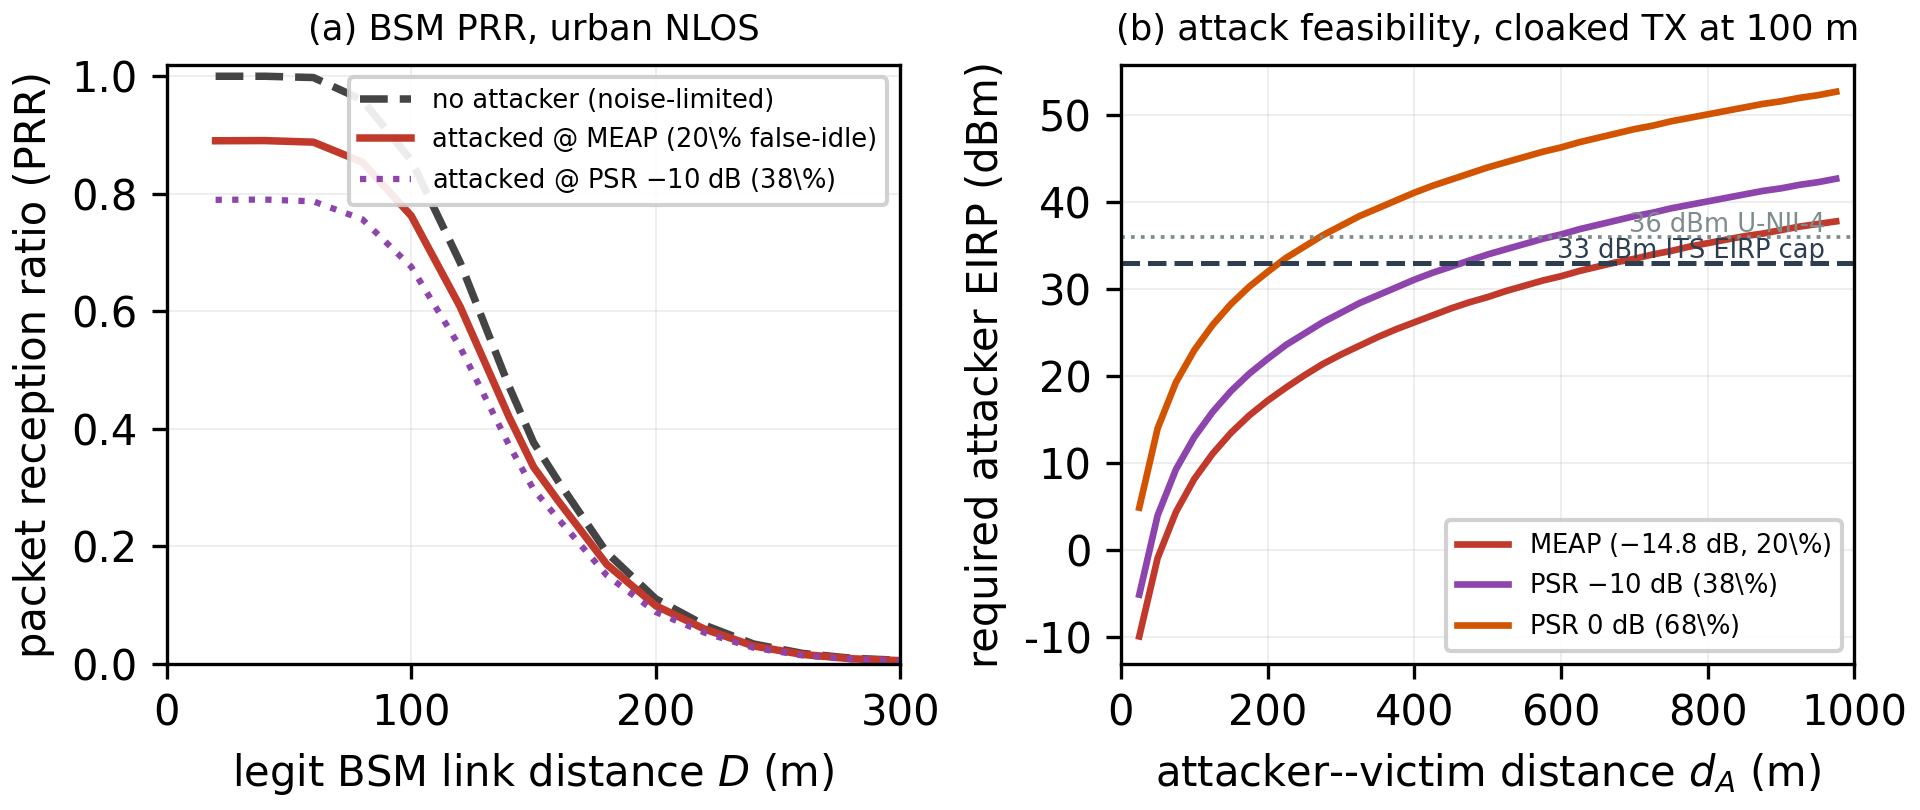
\includegraphics[width=\linewidth]{figs/harm_chain.png}
\caption{The harm chain, urban NLOS parameters. (a) Legitimate BSM PRR
vs.\ link distance without and with the compliant attacker at the
targeted MEAP and $-10$\,dB operating points (synchronized worst-case
timing, no-capture model). (b) Required attacker EIRP vs.\ attacker-
victim distance with the cloaked transmitter at 100\,m; the 33\,dBm ITS
cap makes the attack feasible at hundreds of metres.}
\label{fig:harm}
\end{figure}

This layer is deliberately parametric, not simulated: it is a
link-budget bridge (each parameter standard-textbook, all disclosed,
one Monte-Carlo seed, all curves in \texttt{results/harm\_chain.json}),
not an ns-3 or field campaign---those remain the honest next step, and
the harm numbers should be read as order-of-magnitude quantification of
the consequence, conditional on the measured sensing-level ASR.


\section{Standards, Deployment Implications, and Ethics}
\label{sec:standards}

The compliant-attacker threat model is deliberately aligned with how
spectrum rules are enforced, which makes the results actionable in the
O-RAN and conformance-testing contexts mapped by adversarial-ML threat
analyses~\cite{habler2025}. Five deployment scenarios, stated with their
preconditions and non-claims:

\begin{itemize}
\item \textbf{O-RAN RIC robustness gate:} security engineers run the
released compliant-attack suite against ML-based sensing xApps before
deployment, requiring MEAP above a policy margin; conditional-ASR and PoC
are logged as security KPIs. Single-receiver, differentiable-model scope; no
network-level guarantees.
\item \textbf{FCC transition margin budgeting:} during the 5.9\,GHz
transition~\cite{fcc2020,fcc2024}, vendors and regulators use the
compliant-ASR-vs-PSR curves as worst-case inputs when setting sensing
thresholds and guard strategies for coexistence receivers. Not field
measurements; non-compliant jammers are out of scope.
\item \textbf{ETSI-style conformance extension:} conformance labs replay
standardized mask-compliant adversarial waveforms through channel emulators
into devices under test, complementing EN~302~571 unwanted-emission and
blocking tests~\cite{etsi302571} with receiver-side adversarial robustness
reporting. Not an established test case; not a substitute for OTA.
\item \textbf{Benchmark for the sub-niche:} the released generators,
channels, attack, and metrics with embedded configurations give
attack/defense papers a common substrate---today every paper self-defines
its threat model, blocking comparison.
\item \textbf{Vendor CI regression gate:} ML teams run the mask-constrained
attack nightly on frozen evaluation sets, alerting when MEAP drops or
compliant ASR rises beyond tolerance, catching silent robustness
regressions across model releases. Requires differentiable model export;
minutes of CPU per run at prototype scale.
\end{itemize}

\paragraph{Where such a sensor would actually sit, and at what latency}
Two placement facts must be stated before any deployment claim. First,
no deployed 2026 radio uses learned spectrum sensing: C-V2X Mode-4
resource selection is RSRP/SCI-based and 802.11p channel access is
energy/preamble-based CCA---the threat model of this paper targets
\emph{proposed} sensing architectures (DAA and coexistence receivers,
O-RAN xApps, conformance extensions), and reads as forward-looking risk
analysis, not as a vulnerability of shipping radios. Second, the sensing
decision itself is cheap: re-measured on the Phase-1 pipeline (front-end
STFT included, 86{,}052-parameter victim), median latency is 2.6\,ms per
window on this project's shared 2-vCPU sandbox---$25.8\times$ the
$102.4\,\mu$s window duration (not a continuous-stream rate), but still
$\sim$37 sensing
decisions per 100\,ms TR~37.885 latency budget, and 2.2\,ms amortized at
batch 8. The earlier Phase-0 benchmark of the same architecture measured
0.985\,ms model-only on faster hardware; both numbers are released with
machine context (results/latency\_phase1.json). Latency is not the
bottleneck for this threat model; robustness is.

\paragraph{Responsible disclosure} The attack operates within existing
regulatory power limits and cannot create spectrum violations; the released
code enables defensive evaluation, and the defense section quantifies
mitigation. We release all artifacts so that the threat model can be
audited, extended, and defended against---the standard rationale for
adversarial-ML publications.

\section{Limitations}
\label{sec:limitations}

(1)~Waveforms are synthetic and standard-parameterized, not OTA captures;
pilots, preambles, and higher-order modulations are not modeled.
(2)~The emission mask is idealized: a flat in-band cap (stricter than real
in-band rules, which permit PRB-level concentration) and a hard OOB null;
the $2\times\!\to\!10\times$ cap relaxation shifts the PoC by only
$-0.9$\,dB, and re-running the canonical experiment against the real
ETSI EN 302 571 V1.2.1 Table-7 template moves the compliant MEAP by only
$+0.4$\,dB (Section~\ref{sec:etsimask}), so the allocation constraint
dominates; a PRB-granular in-band model remains future work.
(3)~Channels are TR~37.885-inspired simplifications (first-tap-only Rician,
UMa-flavored urban spread), block-fading within the window---defensible by
Doppler coherence, but approximate.
(4)~The prototype attacker is white-box with perfect CSI and exact knowledge
of the received realization (worst-case upper bound; the CSI-mismatch
variant is released); the canonical numbers use zero-initialized PGD-10,
while the defenses are additionally evaluated under converged adaptive
attack (PGD-50 with 5 restarts, Section~\ref{sec:adaptive})---reported
ASRs at PGD-10 remain lower bounds on the attack side and upper bounds on
the defense side.
(5)~Prototype scale: the undefended headline carries three training seeds
(mask MEAP spread 1.1\,dB) and the adaptive protocol three attack seeds
$\{7,11,22\}$ (grid-identical, per-window captured; the canonical PGD-10
pair covers attack seeds $\{7,11\}$); the adaptive margins are replicated
across three defense training seeds (spread 3.5--5.5\,dB, larger than the
undefended training-seed spread) \emph{and} three attack seeds (spread
0.1--1.3\,dB, $4$--$23\times$ smaller than the defense-seed spread). The
PGD-10 defense readings now span three defense seeds (AT mask MEAP
$-23.1/-19.7/-20.9$\,dB, TRADES $-19.1/-19.2/-18.5$\,dB; the
naive-vs-adaptive gap of $6.9$--$10.4$\,dB holds on every seed).
Confidence intervals are Wilson binomial on per-cell sampling noise plus
paired-bootstrap MEAP/PoC CIs; model-seed variance (1.1\,dB undefended,
3.5--5.5\,dB defended) remains a separate, additive source. Two floors
remain: five defense seeds and a fusion-adaptive attacker are not run.
(6)~The phase-difference stream contributes nothing on this task; the
``phase-aware'' framing of our prior work is retired honestly.
(7)~The adversarially-trained defense's robustness is confined to its
training power range ($-25$ to $-5$\,dB); attacks at parity or above still
succeed. The rural transfer and the PGD-10 TRADES reading are single-seed
(the adaptive margins are 3-seed).
(8)~The real-capture study uses 96 gated bursts from three capture
locations (74 eval / 22 train windows; genie floors resolved to
$-55$\,dB, real-signal PoC $10.2$--$11.9$\,dB with wide Wilson CIs); PC5, 802.11p and the noise class
remain synthetic, and the real class is 802.11 captured at 5240\,MHz
(U-NII-1, same OFDM family as U-NII-4), placed in the unlicensed half of
the window. (9)~The second-victim study shares the receiver front-end, so
it varies the classifier architecture, not the receiver; transfer attacks
still assume a perfect attacker channel. (10)~The PA study uses a
memoryless Rapp model with per-window backoff and output power control;
no measured PA or transmitter chain is involved, PAPR is computed
without oversampling, and the strict/lenient gates are per-FFT-bin
idealizations of 802.11-style masks rather than regulatory measurement
procedures (RBW, detector type). The PA-aware arm demonstrates that the
threat survives this model class, not that any particular hardware
realization would behave identically. (11)~The harm-chain layer of
Section~\ref{sec:harm} is a parametric link-budget analysis anchored to
the measured ASR curve, not a system-level simulation: no MAC queuing,
congestion control, or re-transmission modeling; single Monte-Carlo seed
with $n=4000$ per distance point; PRR figures are conditional on the
stated standard-textbook parameters and should be read as
order-of-magnitude consequence quantification.

\section{Conclusion}
\label{sec:conclusion}

Emission-mask compliance is not a defense: it shifts the adversarial attack
curve on DL ITS-band spectrum sensing by only ${\sim}$5--7\,dB (untargeted)
and 16--18\,dB (targeted cloaking), while an undefended CNN is broken by a
rule-abiding transmitter operating tens of dB below the victim signal. The
legacy feature-space threat model, translated to physical power, overstates
realizable attacks: its own perturbation, made physical, mostly fails, while
a purpose-optimized waveform at the same implied power is far stronger; the
PSR-equivalence translation makes such comparisons meaningful. The
power-amplifier reality check sharpens the regulatory reading: the naive
floating-point-compliant attack is the highest-PAPR signal on the air and
fails a post-PA conformance test at operating backoffs while losing
almost no effectiveness, and a PA-aware re-optimization is both stronger
and post-PA compliant---so compliance testing should sit at the PA
output port, and compliance itself buys detectability of unsophisticated
attackers, not safety against the worst case. The mask idealization
survives contact with four enforcement domains spanning two
administrations (real ETSI EN 302 571 template $+0.4$\,dB; its
RBW/mean-power measurement domain and the US 47~CFR~95.3205-shaped
limits $-0.3$ to $-0.8$\,dB), receiver fusion raises the attack's power
floor by 25\,dB without changing the price of compliance, and
the harm chain closes the gap from sensing error to fleet consequence:
inside ITS power rules, a synchronized attacker at the targeted 20\%
false-IDLE point costs 9.4\,pp of BSM PRR at 100\,m. Two protocol
lessons generalize beyond this paper: defense evaluations that are not
converged (step-starved PGD, no restarts) will systematically overstate
robustness---ours did, by a factor of two---and sensing-level ASR must be
paired with a link-budget layer before it can be called a safety claim.
The compliant-attacker threat
model, the MEAP and Price-of-Compliance metrics, and the released
end-to-end framework give regulators, standards bodies, and O-RAN security
engineers a physically grounded, certification-style way to measure---and,
with mask-matched adversarial training, to
raise---the cost of attacking deep-learning spectrum sensing: $+6.7$\,dB
against a converged adaptive attacker at zero clean-accuracy cost (AT,
canonical defense seed; $+9.8\pm2.8$\,dB across three defense seeds),
$+9.9$\,dB with a TRADES variant at 0.75\,pp clean cost ($+11.5\pm1.8$\,dB
3-seed). The
stress-tests say the same thing in more ways: seed-stable, real-signal-valid,
architecture-discriminating, error-barred, and now adaptive-attack
certified---the numbers move, the conclusions do
not.

% ============================================================================
\begin{thebibliography}{99}

\bibitem{o2018} T. J. O'Shea, T. Roy, T. C. Clancy,
``Over-the-air deep learning based radio signal classification,''
\emph{IEEE J. Sel. Topics Signal Process.}, vol. 12, no. 1, pp. 168--179,
Feb. 2018, doi: 10.1109/JSTSP.2018.2797022.

\bibitem{girmay2023} M. Girmay, V. Maglogiannis, D. Naudts, M. Aslam,
A. Shahid, I. Moerman, ``Technology recognition and traffic characterization
for wireless technologies in ITS band,'' \emph{Vehicular Communications},
vol. 39, art. 100563, Feb. 2023, doi: 10.1016/j.vehcom.2022.100563.

\bibitem{sadeghi2019} M. Sadeghi, E. G. Larsson, ``Adversarial attacks on
deep-learning based radio signal classification,'' \emph{IEEE Wireless
Commun. Lett.}, vol. 8, no. 1, pp. 213--216, Feb. 2019,
doi: 10.1109/LWC.2018.2867459.

\bibitem{kim2020} B. Kim, Y. E. Sagduyu, K. Davaslioglu, T. Erpek,
S. Ulukus, ``Over-the-air adversarial attacks on deep learning based
modulation classifier over wireless channels,'' in \emph{Proc. 54th Annu.
Conf. Information Sciences and Systems (CISS)}, 2020, pp. 1--6,
doi: 10.1109/CISS48834.2020.1570617416.

\bibitem{sagduyu2021} B. Kim, Y. E. Sagduyu, K. Davaslioglu, T. Erpek,
S. Ulukus, ``Channel-aware adversarial attacks against deep learning-based
wireless signal classifiers,'' \emph{IEEE Trans. Wireless Commun.}, vol. 21,
no. 6, pp. 3868--3880, Jun. 2022, doi: 10.1109/TWC.2021.3124855.

\bibitem{liu2022} M. Liu, H. Zhang, Z. Liu, N. Zhao, ``Attacking spectrum
sensing with adversarial deep learning in cognitive radio-enabled Internet of
Things,'' \emph{IEEE Trans. Rel.}, vol. 72, no. 2, pp. 431--444, Jun.
2023, doi: 10.1109/TR.2022.3179491.

\bibitem{zheng2026} S. Zheng, Z. Ye, L. Zhang, K. Yue, Z. Zhao, ``Targeted
adversarial attacks against deep learning-based wideband spectrum sensing,''
\emph{IEEE Trans. Mach. Learn. Commun. Netw.}, vol. 4, pp. 950--965, 2026,
doi: 10.1109/TMLCN.2026.3694666.

\bibitem{radioshock2026} W. Li, C. Li, G. Zhang, Z. Huang, G. Qu, X. Cheng,
J. Luo, P. Hu, ``RadioShock: over-the-air adversarial attacks on wireless
communication,'' \emph{IEEE Trans. Dependable Secur. Comput.}, vol. 23,
no. 4, pp. 8874--8890, 2026, doi: 10.1109/TDSC.2026.3689592.

\bibitem{zhao2024} W. Zhao, X. Li, S. Zhao, J. Xu, Y. Liu, Z. Lu,
``Detecting adversarial spectrum attacks via distance to decision boundary
statistics,'' in \emph{Proc. IEEE INFOCOM}, 2024, pp. 691--700,
doi: 10.1109/INFOCOM52122.2024.10621153.

\bibitem{croce2020} F. Croce, M. Hein, ``Reliable evaluation of adversarial
robustness with an ensemble of diverse parameter-free attacks,'' in
\emph{Proc. 37th Int. Conf. Machine Learning (ICML)}, PMLR, vol. 119, 2020,
pp. 2206--2216.

\bibitem{habler2025} E. Habler, R. Bitton, D. Avraham, E. Klevansky,
D. Mimran, O. Brodt, H. Lehmann, Y. Elovici, A. Shabtai, ``Adversarial
machine learning threat analysis and remediation in Open Radio Access
Network (O-RAN),'' \emph{J. Netw. Comput. Appl.}, vol. 236, art. 104090,
Apr. 2025, doi: 10.1016/j.jnca.2024.104090.

\bibitem{fcc2020} Federal Communications Commission, ``Use of the
5.850--5.925~GHz Band,'' First Report and Order, FCC 20-164, ET Docket
No. 19-138, adopted Nov. 18, 2020 (published at 86 FR 23281, May 3, 2021).

\bibitem{fcc2024} Federal Communications Commission, ``Use of the
5.850--5.925~GHz Band,'' Second Report and Order, FCC 24-123, ET Docket
No. 19-138, adopted Nov. 20, 2024 (published at 89 FR 100838, Dec. 13,
2024; effective Feb. 11, 2025).

\bibitem{itsa2024} ITS America, ``Future of V2X in 5.9~GHz Report,''
May 2024. [Online]. Available:
https://itsa.org/wp-content/uploads/2024/05/ITS-America-Future-of-V2X-in-5.9-GHz-Report.pdf

\bibitem{5gaa2024} 5G Automotive Association (5GAA), ``C-V2X roadmap
update,'' Dec. 2024.

\bibitem{anand2008} S. Anand, Z. Jin, K. P. Subbalakshmi, ``An analytical
model for primary user emulation attacks in cognitive radio networks,'' in
Proc. 3rd IEEE Symp. New Frontiers in Dynamic Spectrum Access Networks
(DySPAN), Chicago, IL, Oct. 2008, pp. 1--12.

\bibitem{ambhika2024} C. Ambhika, ``Discrimination of primary user
emulation attack on cognitive radio networks using machine learning based
spectrum sensing scheme,'' Wireless Networks, vol. 30, no. 5, Oct. 2024.

\bibitem{etsi302571} ETSI, ``Intelligent Transport Systems (ITS);
Radiocommunications equipment operating in the 5~855~MHz to 5~925~MHz
frequency band; Harmonised Standard covering the essential requirements of
article 3.2 of Directive 2014/53/EU,'' ETSI EN 302 571, V1.2.1, Sep. 2013.
Mask values used in Section~\ref{sec:etsimask} are extracted from the
official PDF (sha256 667a939\ldots) and committed as machine-readable
tables with provenance (\texttt{data/standards/en302571\_tables.json}).

\bibitem{tr37885} 3GPP, ``Study on evaluation methodology of new
Vehicle-to-Everything (V2X) use cases for LTE and NR,'' 3GPP TR 37.885,
V15.3.0, Release 15, Jun. 2019.

\bibitem{ts36211} 3GPP, ``Evolved Universal Terrestrial Radio Access
(E-UTRA); Physical channels and modulation,'' 3GPP TS 36.211, V15.14.0,
Release 15, Oct. 2021.

\bibitem{ieee80211} IEEE, ``IEEE Standard for Information
technology---Telecommunications and information exchange between
systems---Local and metropolitan area networks---Specific
requirements---Part 11: Wireless LAN Medium Access Control (MAC) and
Physical Layer (PHY) Specifications,'' IEEE Std 802.11-2012, 2012.

\bibitem{dhankhar2026} P. Dhankhar, D. Vats, ``Dual-stream phase-aware
Inception-Time CNN for adversarially robust spectrum sensing in V2X
networks,'' in \emph{Proc. Int. Conf. Computing, Communication, and
Technologies (ICE2CT)}, 2026.

\end{thebibliography}

\end{document}
